\chapter{Livello trasporto}

\section{Introduzione}
Il livello trasporto si colloca fra il livello rete e il livello applicazione, e fornisce un servizio di comunicazione tra processi fra i due livelli applicazione, uno sull'host locale e l'altro sull'host remoto. Il servizio di comunicazione viene fornito tramite una connessione logica, che consente ai due livelli applicazione (che possono essere situati in qualsiasi parte del mondo) di lavorare come se ci fosse una connessione diretta attraverso la quale inviare e ricevere i messaggi.

\begin{Example}{Livello trasporto}{}
    \begin{minipage}[c]{0.55\textwidth}
        L'host di Gaia nell'azienda Sky Research crea una connessione logica a livello trasporto con l'host di Gabriele nell'azienda Scientific Books. Le due aziende comunicano a livello trasporto come se fra di loro esistesse un canale di comunicazione reale. Da notare che solamente i due sistemi finali (i computer di Gabriele e di Gaia) usano i servizi del livello trasporto, mentre i router intermedi utilizzano solo i primi tre livelli dell'architettura di rete.
    \end{minipage}
    \hfill
    \begin{minipage}[c]{0.44\textwidth}
        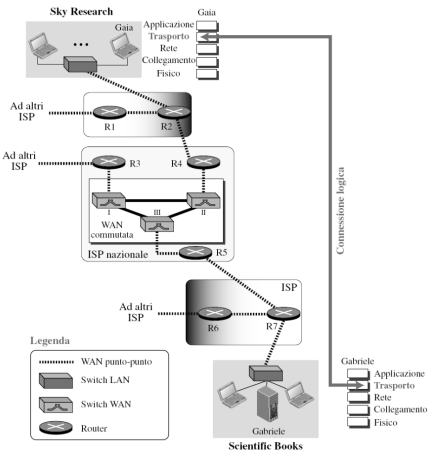
\includegraphics[width=1\textwidth]{images/trasporto.PNG}
    \end{minipage}    
\end{Example}

\subsection{I servizi del livello trasporto}
Il livello trasporto si colloca fra il livello rete e il livello applicazione: fornisce quindi servizi al livello applicazione e riceve servizi dal livello rete.

\subsubsection*{Comunicazione tra processi}
Il primo compito di un protocollo di livello trasporto è supportare la comunicazione tra processi. Un processo è un'entità (programma in esecuzione) di livello applicazione che usa i servizi del livello trasporto. Prima di descrivere la comunicazione tra processi, vediamo la comunicazione tra host.

Il livello rete si occupa della comunicazione tra dispositivi, ovvero della comunicazione tra host. Un protocollo di rete consegna i messaggi al computer destinatario, ma questo tipo di consegna è incompleta, perché i messaggi devono giungere ai processi cui erano indirizzati (sullo stesso host possono essere attivi svariati processi applicativi). E' a questo punto che intervengono i protocolli del livello trasporto, che completano la consegna passando i messaggi ai processi applicativi destinatari.

\begin{figure}[ht]
    \centering
    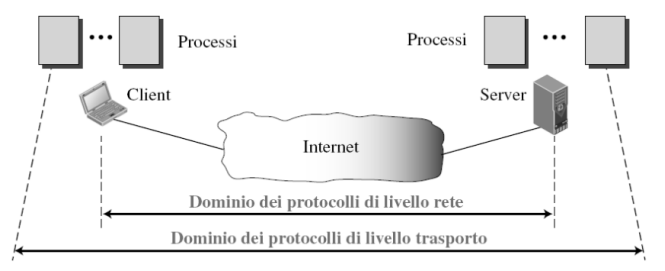
\includegraphics[width=9cm]{images/trasporto-e-rete.PNG}
    \caption{Livello rete e livello trasporto a confronto}
    \label{fig:trasp-e-rete}
\end{figure}

\subsubsection*{Indirizzamento: i numeri di porta}
Sebbene la comunicazione tra processi possa essere realizzata in diversi modi, la più diffusa è sicuramente quella basata sul paradigma client/server. Un processo sulla macchina locale, il client, necessita di servizi svolti da un processo solitamente su una macchina remota, il server. Va osservato, però, che la maggior parte dei sistemi operativi attuali è multiutente e multiprocesso, quindi l'host locale ha spesso diversi processi client attivi, così come l'host remoto può avere diversi processi server attivi. Affinché si possa stabilire una comunicazione tra i due dispositivi, è necessario un metodo per individuare: l'host locale, l'host remoto, il processo locale e il processo remoto. Gli host vengono individuati per mezzo del loro indirizzo IP.

Al client viene assegnato un numero di porta che viene detto effimero, ovvero "di breve durata", dato il breve tempo di vita di un processo client.

Anche al server deve essere associato un numero di porta, che, però, non può essere scelto a caso, perché tale numero deve essere in qualche modo noto al client. Una soluzione potrebbe essere l'invio di un pacchetto al fine di scoprire questo numero di porta, ma ciò creerebbe un carico inutile sulla rete. Nei protocolli TCP/IP si usano numeri universali per i server, che sono detti numeri di porta noti (well-known). Ogni client conosce il numero di porta noto del server corrispondente. Per esempio, mentre il client Daytime può usare il numero di porta effimero 52000, il server Daytime deve usare necessariamente il numero di porta noto 13.

\begin{figure}[ht]
    \centering
    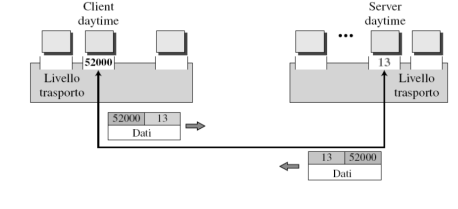
\includegraphics[width=0.5\textwidth]{images/numeri-porta.PNG}
    \hfill
    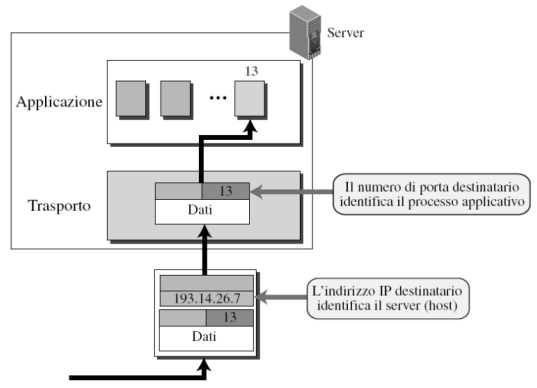
\includegraphics[width=0.45\textwidth]{images/IP-e-numporta.PNG}
    \caption{Numeri di porta}
    \label{fig:numeri-porta}
\end{figure}

Deve essere chiaro che gli indirizzi IP e i numeri di porta giocano ruoli ben distinti nel selezionare la destinazione finale. L'indirizzo IP individua un host tra gli innumerevoli host di tutta la rete mondiale; il numero di porta individua uno dei processi applicativi del particolare host individuato dall'indirizzo IP.

\subsubsection*{Incapsulamento/decapsulamento}
Per inviare un messaggio da un processo a un altro, il protocollo di livello trasporto incapsula e decapsula i messaggi. L'incapsulamento avviene dal lato del mittente. Quando un processo deve inviare un messaggio, lo passa al livello trasporto insieme ad altre informazioni, che dipendono dal protocollo del livello trasporto. Il livello trasporto riceve i dati e vi aggiunge la propria intestazione (incapsulando il messaggio applicativo in un pacchetto del livello trasporto). I pacchetti a livello trasporto sono chiamati segmenti (nel protocollo TCP) o datagrammi utente (nel protocollo UDP).

Il decapsulamento avviene dal lato del destinatario. Quando il messaggio arriva al livello trasporto del destinatario, l'intestazione viene rimossa e il messaggio (decapsulato) viene consegnato al processo a livello applicazione.

\begin{figure}[ht]
    \centering
    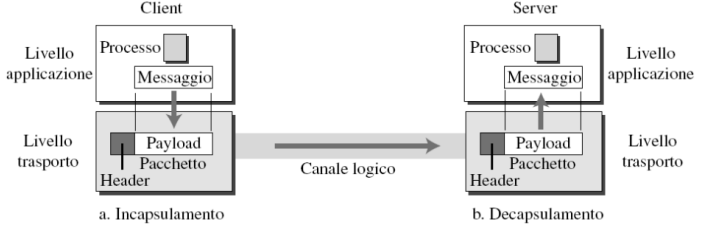
\includegraphics[width=10cm]{images/incaps-decaps-tra.PNG}
    \caption{Incapsulamento e decapsulamento}
    \label{fig:incaps-decaps-tra}
\end{figure}

\subsubsection*{Multiplexing e demultiplexing}
Il termine multiplexing (molti a uno) fa riferimento al caso in cui un'entità riceve informazioni da più di una sorgente, il termine demultiplexing fa riferimento al caso in cui un'entità trasmette informazioni a più di un destinatario. Il livello trasporto effettua il multiplexing nel sito mittente e il demultiplexing nel sito destinatario.

\begin{Example}{Multiplexing e demultiplexing}{}
    \textit{Tre processi client, P1, P2 e P3, sono in esecuzione su un host. I processi P1 e P3 devono inviare delle richieste al processo server corrispondente, in esecuzione su un server. Il processo client P2 deve inviare una richiesta al processo server corrispondente in esecuzione su un altro server.}
    
    \begin{minipage}[c]{0.55\textwidth}
        Il livello trasporto nel client accetta i tre messaggi dai tre processi e crea tre pacchetti: agisce da multiplexer. I pacchetti 1 e 3 usano lo stesso canale logico per raggiungere il livello trasporto del primo server. Quando arrivano al server, il livello trasporto agisce da demultiplexer distribuendo i messaggi a due processi differenti. Il livello trasporto nel secondo server riceve il pacchetto 2 e lo consegna al processo corrispondente. Si noti che anche in questo caso si ha comunque un'operazione di demultiplexing sebbene vi sia un solo messaggio.
    \end{minipage}
    \hfill
    \begin{minipage}[c]{0.44\textwidth}
        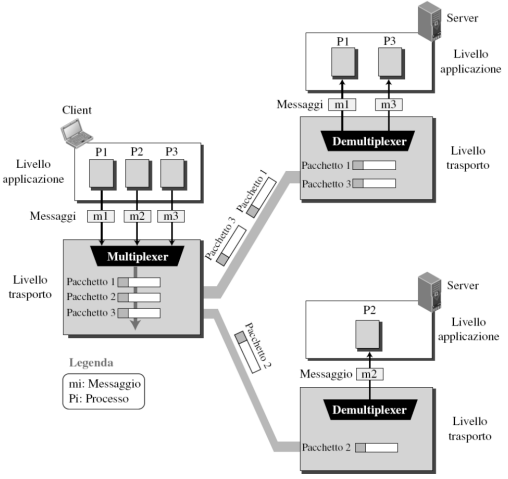
\includegraphics[width=1\textwidth]{images/mult-demul-tra.PNG}
    \end{minipage}
\end{Example}

\begin{Example}{Multiplexing e demultiplexing}{}
    \textit{Supponiamo che vi troviate di fronte al vostro computer e che stiate scaricando pagine web mentre sono in esecuzione una sessione FTP e due sessioni Telnet. Avrete pertanto quattro processi applicativi in esecuzione: due Telnet, uno FTP e uno HTTP.} 

    \begin{minipage}{\textwidth}
        \centering
        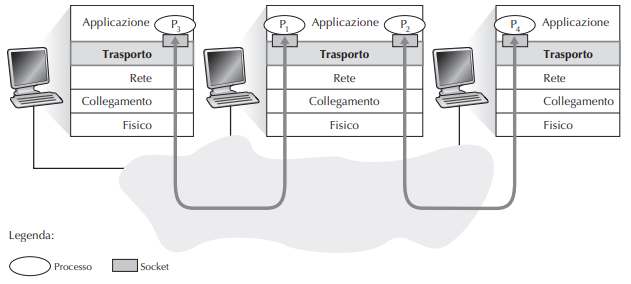
\includegraphics[width=0.7\linewidth]{images/es-mult-demul-tra.PNG}
        %\captionof{figure}{Esempio}
    \end{minipage}

    Il livello di trasporto nel vostro calcolatore, quando riceve dati dal livello di rete sottostante, li deve indirizzare a uno di questi quattro processi. Di conseguenza il livello di trasporto nell'host di ricezione in realtà non trasferisce i dati direttamente a un processo, ma piuttosto a una socket che fa da intermediario. Siccome, a ogni dato istante, può esserci più di una socket nell'host di ricezione, ciascuna avrà un identificatore univoco il cui formato dipende dal fatto che si tratti di socket UDP o TCP.
    
    Il compito di trasportare i dati dei segmenti a livello di trasporto verso la giusta socket viene detto demultiplexing. Il compito di radunare frammenti di dati da diverse socket sull'host di origine e incapsulare ognuno con intestazioni a livello di trasporto (che verranno poi utilizzate per il demultiplexing) per creare dei segmenti e passarli al livello di rete, viene detto multiplexing. 
    
    Si noti che il livello di trasporto nell'host centrale deve effettuare il demultiplexing dal livello di rete di segmenti che possono arrivare sia per il processo P1 sia per P2; ciò avviene indirizzando i dati del segmento in ingresso alla giusta socket. Il livello di trasporto nell'host centrale deve, inoltre, raccogliere i dati in uscita dalle socket dei due processi, creare i segmenti a livello di trasporto e passarli al livello di rete.
\end{Example}

\begin{wrapfigure}{r}{0.30\textwidth}
    \vspace{-0.5cm}
    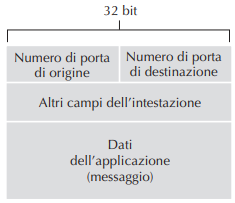
\includegraphics[width=0.27\textwidth]{images/campi-trasporto.PNG}
    \vspace{-0.5cm}
    %\caption{Birds}
\end{wrapfigure}
    
Ora che abbiamo compreso i ruoli del multiplexing e del demultiplexing a livello di trasporto esaminiamo come vengono realizzati negli host. Da quanto visto in precedenza, sappiamo che il multiplexing a livello di trasporto richiede (1) che le socket abbiano identificatori unici e (2) che ciascun segmento presenti campi che indichino la socket cui va consegnato il segmento. Questi sono il campo del numero di porta di origine e il campo del numero di porta di destinazione. I numeri di porta sono di 16 bit e vanno da 0 a 65535, quelli che vanno da 0 a 1023 sono chiamati numeri di porta noti (well-known port number) e sono riservati per essere usati da protocolli applicativi ben noti quali HTTP (porta 80) e FTP (porta 21).

\begin{Example}{Numero di porta}{}
    \begin{minipage}{\textwidth}
        \centering
        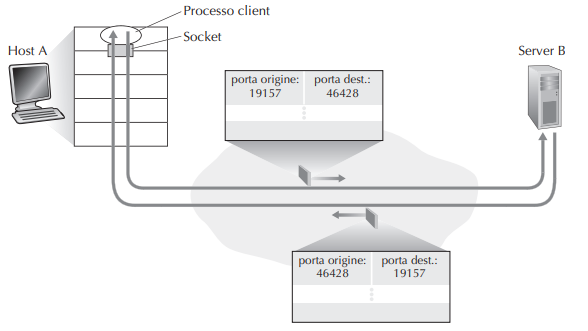
\includegraphics[width=0.7\linewidth]{images/n-porta-origin.PNG}
        %\captionof{figure}{Esempio}
    \end{minipage}
    
    Per quanto riguarda il numero di porta nel segmento che va da A verso B, il numero di porta di origine serve come parte di un “indirizzo di ritorno”: quando B vuole restituire il segmento ad A, la porta di destinazione del segmento da B verso A assumerà il valore della porta di origine del segmento da A verso B. L'indirizzo di ritorno completo è costituito dall'indirizzo IP di A più il numero di porta di origine.    
\end{Example}

\subsection{API di comunicazione}
Come può un processo client comunicare con un processo server? Se si vuole sviluppare un programma capace di comunicare con un altro programma, è necessario un nuovo insieme di istruzioni per chiedere ai primi quattro livelli dello stack TCP/IP di aprire la connessione, inviare/ricevere dati e chiudere la connessione. Un insieme di istruzioni di questo tipo viene chiamato API (Application Programming Interface). Nella programmazione, un'interfaccia non è altro che un insieme di istruzioni usato per l'interazione tra due entità. In questo caso una delle entità è il processo a livello applicazione e l'altra è il sistema operativo che implementa i primi quattro livelli dello stack TCP/IP. Sono state sviluppate diverse API di comunicazione, tra le quali tre sono le più note: l'interfaccia socket (socket interface), TLI (Transport Layer Interface) e STREAMS.

\begin{figure}[ht]
    \centering
    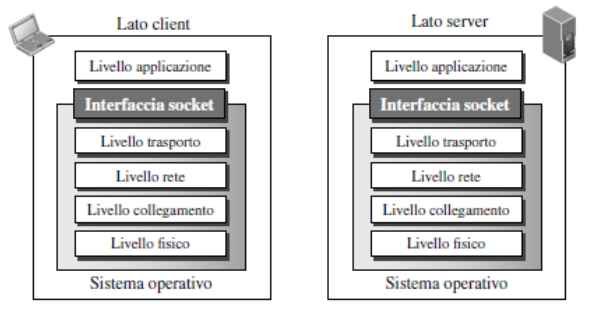
\includegraphics[width=10cm]{images/api-comunic.PNG}
    \caption{L'interfaccia socket nella pila dei protocolli}
    \label{fig:incaps-decaps-tra}
\end{figure}

\subsubsection*{Socket}
l'interfaccia socket è un insieme di istruzioni che consentono la comunicazione fra il livello applicazione e il sistema operativo; è un insieme di istruzioni che possono essere utilizzate da un processo per comunicare con un altro processo.

Sebbene una socket possa apparire come un terminale o un file, non è un'entità fisica di questo tipo: è un'astrazione. Si tratta in realtà di una struttura dati creata e utilizzata dal programma applicativo. Si può dire che, per quanto riguarda il livello applicazione, comunicare fra un processo client e un processo server significa comunicare tra due socket create nei due lati della comunicazione.

\begin{figure}[ht]
    \centering
    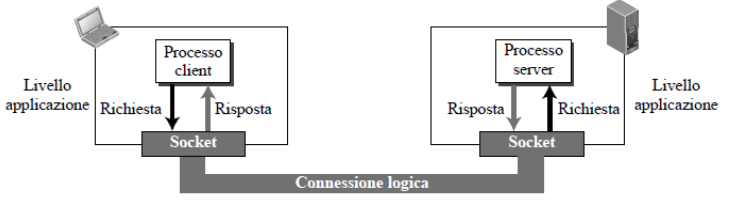
\includegraphics[width=11cm]{images/socket.PNG}
    \caption{Impiego delle socket nella comunicazione tra processi}
    \label{fig:socket}
\end{figure}

Il client considera la socket come l'entità che riceve le richieste e fornisce le risposte; il server vede la socket come l'entità che gli sottopone le richieste e alla quale inviare le risposte. Se si creano due socket, una a ciascun lato della comunicazione, definendo correttamente gli indirizzi mittente e destinatario, si possono utilizzare tutte le istruzioni disponibili per inviare e ricevere dati.

\subsubsection*{Socket address}
L'interazione fra client e server è una comunicazione bidirezionale. Nella comunicazione bidirezionale si rende necessaria una coppia di indirizzi: locale (mittente) e remoto (destinatario). L'indirizzo locale in una direzione è l'indirizzo remoto nell'altra direzione e viceversa. Poiché la comunicazione nel paradigma client/server avviene fra due socket, è necessaria una coppia di socket address (indirizzi delle socket) per la comunicazione: un socket address locale ed uno remoto.

\begin{wrapfigure}{r}{0.40\textwidth}
    \vspace{-0.5cm}
    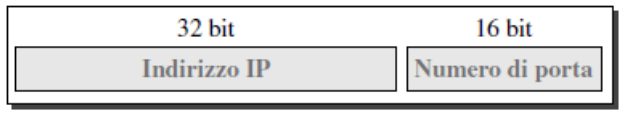
\includegraphics[width=0.37\textwidth]{images/socket-address.PNG}
    \vspace{-0.4cm}
    %\caption{Birds}
\end{wrapfigure}

Un socket address deve innanzitutto identificare l'host sul quale il processo client o server è in esecuzione, definito univocamente dal proprio indirizzo IP, che solitamente è un intero a 32 bit. Ma sullo stesso computer potrebbero essere eseguiti contemporaneamente diversi processi client o server, di conseguenza è necessario utilizzare un altro identificatore per specificare il particolare client o server coinvolto nella comunicazione: il numero di porta, un intero a 16 bit. Un socket address sarà quindi composto dalla combinazione di un indirizzo IP e un numero di porta.

Dato che una socket specifica gli end-point (estremi) della comunicazione, è possibile affermare che una socket è identificata da una coppia di socket address, uno locale e uno remoto.

\subsubsection*{Individuare i socket address}
Come può un client o un server individuare la coppia di socket address per effettuare la comunicazione? La situazione è differente a seconda del lato della comunicazione.

\begin{itemize}
    \item \textit{Lato server.} Il server ha bisogno di un socket address locale (server) e un socket address remoto (client) per comunicare.

    Il socket address locale (server) viene fornito dal sistema operativo. Il sistema operativo conosce l'indirizzo IP del computer sul quale il processo server è in esecuzione. Il numero di porta di un processo server, invece, deve essere assegnato.

    Il socket address remoto di un server è il socket address del client che si collega. Poiché il server può servire numerosi client, non può conoscere in anticipo il loro l'indirizzo, ma lo può identificare quando un client cerca di connettersi. Il socket address del client, contenuto nel pacchetto di richiesta inviato al server, diviene il socket address remoto utilizzato per rispondere al client. 
    
    Il socket address locale di un server è fissato e rimane invariato, mentre il socket address remoto varia a ogni interazione con un client differente.

    \item \textit{Lato client.} Per comunicare, anche il client ha bisogno di due socket address, uno locale e uno remoto. 
    
    Anche il socket address locale (client) viene fornito dal sistema operativo, che conosce l'indirizzo IP del computer sul quale è in esecuzione il client. Il numero di porta invece è un intero di 16 bit che viene assegnato temporaneamente al client ogni volta che questo desidera iniziare una comunicazione. Il numero di porta deve essere scelto fra un insieme di interi definiti dagli enti di gestione di Internet chiamati numeri di porta effumeri (o temporanei). Il sistema operativo deve garantire che il numero di porta così assegnato non sia utilizzato da alcun altro processo client contemporaneamente in esecuzione.

    Individuare il socket address remoto (server) comporta operazioni un pò più complesse. Un processo client, quando viene avviato, deve conoscere il socket address del server al quale vuole connettersi. Si hanno due possibili situazioni.

    \begin{enumerate}
        \item In alcuni casi l'utente che avvia il processo client conosce sia il numero di porta che l'indirizzo IP del computer sul quale è in esecuzione il server.
        \item Sebbene tutte le applicazioni standard abbiano un numero di porta noto, nella maggior parte dei casi non si conosce l'indirizzo IP: il processo client solitamente conosce il numero di porta, trattandosi di un numero di porta noto, mentre l'indirizzo IP può essere ottenuto utilizzando un'altra applicazione client/ server chiamata DNS (Domain Name System).
    \end{enumerate}
\end{itemize}

\subsection{Protocolli Internet di livello trasporto}
Avendo discusso i concetti generali relativi al livello trasporto, si approfondiscono ora due dei protocolli di livello trasporto impiegati in Internet, UDP e TCP. Questi protocolli sono situati fra il livello applicazione e il livello rete e agiscono da intermediari fra i programmi applicativi e le operazioni della rete.

UDP è un protocollo di trasporto inaffidabile e privo di connessione, utilizzato per la sua semplicità ed efficienza nei casi in cui il controllo degli errori può essere gestito dai processi di livello applicazione. TCP è un protocollo affidabile, orientato alla connessione, che può essere utilizzato nelle applicazioni dove l'affidabilità è particolarmente importante.

\section{Protocollo UDP (User Datagram Protocol)}
UDP (User Datagram Protocol) è un protocollo del livello trasporto inaffidabile e privo di connessione. Non aggiunge nulla ai servizi di IP eccetto la comunicazione tra processi. Per quale motivo un processo dovrebbe utilizzare UDP, se offre così pochi servizi? Gli svantaggi hanno come contropartita alcuni vantaggi. UDP è un protocollo molto semplice con un overhead (carico aggiuntivo) minimo. Se un processo vuole inviare un piccolo messaggio senza doversi preoccupare troppo dell'affidabilità, si può utilizzare UDP. Inviare un messaggio con UDP richiede meno interazioni fra il mittente e il destinatario rispetto all'impiego del TCP.

Il mittente invia pacchetti uno dopo l'altro senza pensare al destinatario (può inviare dati a raffica perché non c'è controllo di flusso né di congestione).

\begin{figure}[ht]
    \centering
    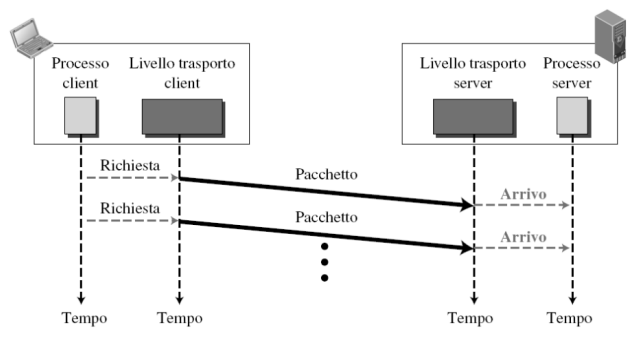
\includegraphics[width=10cm]{images/udp.PNG}
    \caption{Diagramma di comunicazione}
    \label{fig:udp}
\end{figure}

Il mittente deve dividere i suoi messaggi in porzioni di dimensioni accettabili dal livello di trasporto, a cui consegnarli uno per uno. Ogni pacchetto è indipendente dagli altri (la sequenza di arrivo può essere diversa da quella di spedizione). Non c'è coordinazione tra livello trasporto mittente e destinatario. Non è possibile implementare efficacemente controllo di flusso, controllo degli errori, controllo della congestione.

\begin{figure}[ht]
    \centering
    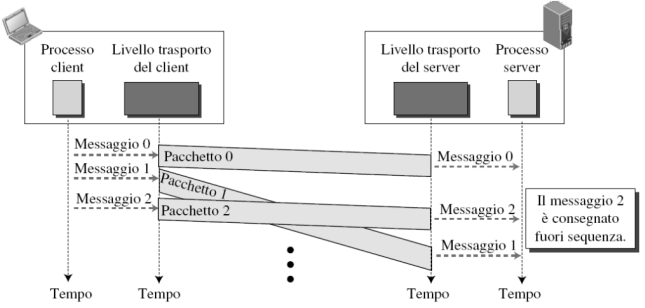
\includegraphics[width=10cm]{images/udp2.PNG}
    \caption{Servizi privi di connessione}
    \label{fig:udp2}
\end{figure}

Il comportamento di un protocollo di trasporto può essere rappresentato da un automa a stati finiti. L'automa rimane in uno stato fin quando non avviene un evento che può modificare le stato dell'automa (transizione di stato) e fargli compiere un'azione.

\subsection{Protocollo semplice}
Un primo protocollo semplice, privo di connessione, senza controllo degli errori e del flusso suppone che il destinatario sa in grado di gestire immediatamente tutti i pacchetti ricevuti; in altri termini, il destinatario non viene mai sovraccaricato dai pacchetti in arrivo.

\begin{figure}[ht]
    \centering
    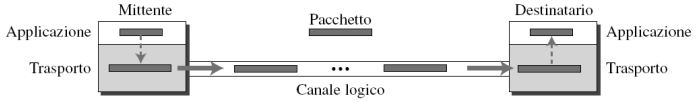
\includegraphics[width=11cm]{images/udp3.PNG}
    \caption{Protocollo semplice}
    \label{fig:udp3}
\end{figure}

Il livello trasporto mittente riceve un messaggio dal proprio livello applicazione, ne crea un pacchetto e lo invia. Il livello trasporto destinatario riceve il datagramma dal proprio livello rete, ne estrae il messaggio e lo consegna al proprio livello applicazione. I livelli trasporto del mittente e del destinatario forniscono quindi servizi di comunicazione ai rispettivi livelli applicazione.

Il mittente non può inviare pacchetti fino a quando il suo livello applicazione non ha un messaggio da spedire. Analogamente il destinatario non può consegnare un messaggio al proprio livello applicazione fino a quando non riceve un pacchetto. E' possibile rappresentare questi due vincoli usando due FSM, ognuna costituita dal solo stato ready (pronto). La macchina mittente rimane nello stato ready fino a quando arriva una richiesta dal processo nel livello applicazione. Quando avviene questo evento, la macchina mittente incapsula il messaggio in un pacchetto e lo invia alla macchina destinataria. La macchina destinataria rimane nello stato ready fino a quando non arriva un pacchetto dal mittente. Quando avviene questo evento, la macchina destinataria estrae il messaggio dal pacchetto e lo consegna al processo nel livello applicazione.

\begin{figure}[ht]
    \centering
    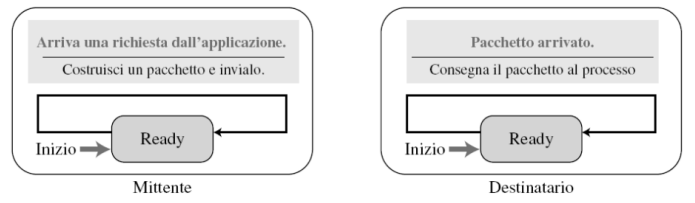
\includegraphics[width=10cm]{images/fsm-udp.PNG}
    \caption{FSM per il protocollo semplice}
    \label{fig:fsm-udp}
\end{figure}

\subsection{Struttura dei datagrammi utente}
I pacchetti UDP sono chiamati datagrammi utente; la loro intestazione è costituita da 4 campi di 2 byte (16 bit) per un totale di 8 byte fissi. I primi due campi definiscono i numeri di porta di mittente e destinatario. Il terzo campo definisce la lunghezza totale, intestazione più dati, del datagramma utente. I 16 bit possono definire una lunghezza totale da 0 a 65535 byte, ma in realtà la dimensione è inferiore perché il datagramma utente UDP viene inserito in un datagramma IP con lunghezza totale di 65535 byte. L'ultimo campo può contenere il checksum opzionale.

\begin{figure}[ht]
    \centering
    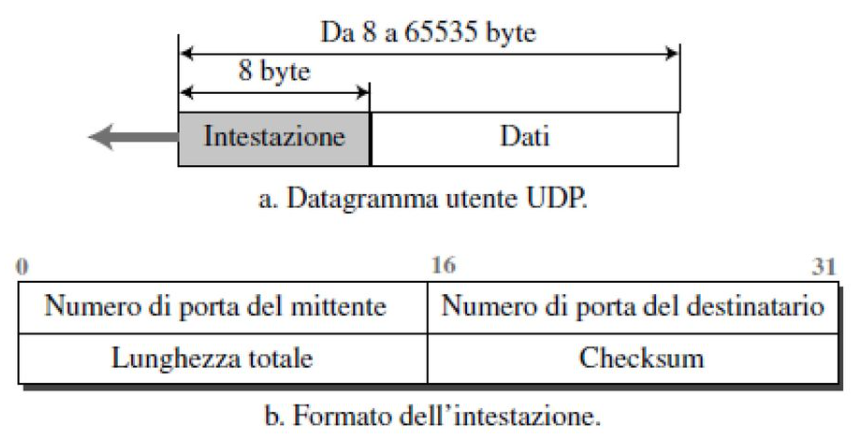
\includegraphics[width=8cm]{images/datagramma-utente.PNG}
    \caption{Formato dei datagramma utente}
    \label{fig:datagramma-utente}
\end{figure}

\subsection{Servizi UDP}
\subsubsection*{Checksum}
Il checksum UDP serve per il rilevamento degli errori. In altre parole, viene utilizzato
per determinare se i bit del segmento UDP sono stati alterati durante il loro trasferimento (per esempio, a causa di disturbi nei collegamenti o quando sono stati memorizzati in un router) da sorgente a destinazione. Lato mittente UDP effettua il complemento a 1 della somma di tutte le parole da 16 bit nel segmento, e l'eventuale riporto finale viene sommato al primo bit. Tale risultato viene posto nel campo checksum del segmento UDP.

\begin{Example}{Calcolo del checksum}{}
    \textit{Calcolare il checksum della seguente stringa di 32 bit:} \verb|11100110011001101101010101010101|.

    Viene effettuata la somma tra le due metà e il riporto viene sommato al primo bit:
    \begin{equation*}
    \begin{array}{cc}
        1110011001100110 & +\\
        1101010101010101 & =\\
        \cline{1-2}
        \rule[0mm]{0cm}{5mm}
        11011101110111011&\\
         \cline{1-2}
        \rule[0mm]{0cm}{5mm}
        1011101110111100
    \end{array}
    \end{equation*}
    Il complemento a 1 si ottiene convertendo i bit 0 in 1 e viceversa. Di conseguenza, il checksum sarà:
    \begin{equation*}
        0100010001000011
    \end{equation*}
\end{Example}

\subsubsection*{DNS usa UDP}
DNS è un tipico esempio di protocollo a livello applicativo che utilizza UDP. Quando l'applicazione DNS in un host vuole effettuare una query, costruisce un messaggio di query DNS e lo passa a UDP. L'entità UDP in esecuzione sul sistema di destinazione aggiunge i campi d'intestazione al messaggio e trasferisce il segmento risultante al livello di rete. Quest'ultimo incapsula il segmento UDP in un datagramma e lo invia a un server DNS. L'applicazione DNS sull'host che ha effettuato la richiesta aspetta quindi una risposta. Se non ne riceve (magari perché la rete sottostante ha smarrito la richiesta o la risposta), l'applicazione tenta di inviare la richiesta a un altro DNS server oppure informa l'applicazione dell'impossibilità di ottenere una risposta. La semplicità della richiesta/risposta (molto breve) motiva l'utilizzo di UDP, che risulta più veloce. UDP è utilizzato anche perché consente un controllo più sottile a livello di applicazione su quali dati sono inviati e quando.

\section{Protocollo TCP (Trasmission Control Protocol)}
Il protocollo TCP (Transmission Control Protocol) è un protocollo orientato alla connessione e affidabile. Per fornire un servizio orientato alla connessione TCP prevede esplicitamente i meccanismi di apertura della connessione, di trasferimento dei dati e di chiusura della connessione. Per fornire un servizio affidabile utilizza una combinazione di meccanismi GBN e SR, con il checksum per la rilevazione degli errori, la ritrasmissione dei segmenti smarriti o corrotti, la conferma cumulativa e selettiva e opportuni timer. TCP è il protocollo di livello trasporto più utilizzato in Internet.

Il protocollo TCP fornisce un servizio di trasporto affidabile tra processi basato, come per UDP, sui numeri di porta. Analogamente a UDP, TCP effettua il multiplexing in trasmissione e il demultiplexing in ricezione. A differenza di UDP, TCP è un protocollo orientato alla connessione, pertanto è necessario stabilire una connessione per ogni coppia di processi prima di avviare la comunicazione tra processi.
Oltre ad essere orientato alla connessione, il protocollo TCP è anche orientato al flusso di dati (stream-oriented), ovvero permette al livello applicazione di trasmettere un flusso di dati.

\begin{figure}[ht]
    \centering
    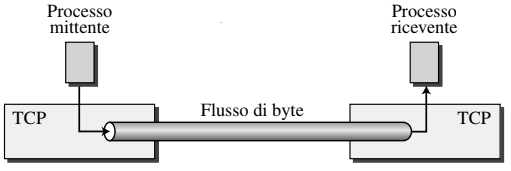
\includegraphics[width=8cm]{images/tcp-tra.PNG}
    \caption{Trasmissione di un flusso}
    \label{fig:tcp-tra}
\end{figure}

\subsection{Servizi TCP}
\subsubsection*{Demultiplexing orientato alla connessione}
Una socket TCP è identificata da quattro parametri: indirizzo IP di origine, numero di porta di origine, indirizzo IP di destinazione e numero di porta di destinazione. Pertanto, quando un segmento TCP giunge dalla rete in un host, quest'ultimo utilizza i quattro valori per dirigere (fare demultiplexing) il segmento verso la socket appropriata. In particolare, due segmenti TCP in arrivo, aventi indirizzi IP di origine o numeri di porta di origine diversi, vengono diretti a due socket differenti, anche a fronte di indirizzo IP e porta di destinazione uguali, con l'eccezione dei segmenti TCP che trasportano la richiesta per stabilire la connessione.

L'host server può ospitare più socket TCP contemporanee collegate a processi diversi, ognuna identificata da una specifica quaterna di valori.

\begin{Example}{Demultiplexing orientato alla connessione}{}
     \textit{L'Host C dà inizio a due sessioni HTTP verso il server B, mentre l'Host A apre una sessione verso B. Gli Host A e C e il server B hanno ciascuno il proprio indirizzo IP, indicati rispettivamente con A, C e B. L'Host C assegna due diversi numeri di porta di origine (26145 e 7532) alle sue due connessioni HTTP.}

     \begin{minipage}{\textwidth}
        \centering
        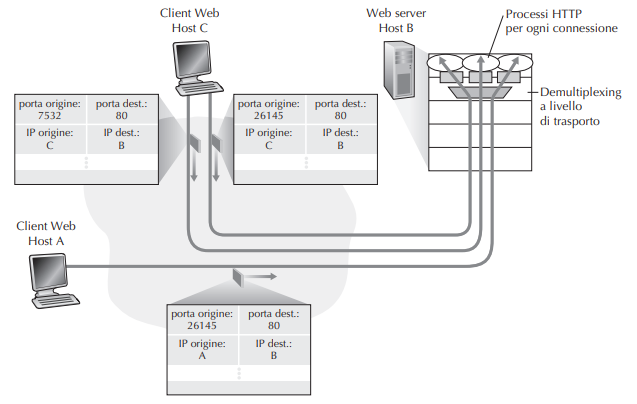
\includegraphics[width=0.7\linewidth]{images/es-demu-conn.PNG}
        %\captionof{figure}{Esempio}
    \end{minipage}
     
     Dato che l'Host A sta scegliendo i numeri di porta di origine indipendentemente da C, potrebbe anch'esso attribuire una porta di origine 26145 alla sua connessione HTTP. Ma questo non è un problema: il server B sarà ancora in grado di fare correttamente demultiplexing delle due connessioni che, pur avendo lo stesso numero di porta di origine, hanno indirizzi IP differenti.
\end{Example}

\subsubsection*{Servizio orientato alla connessione}
In un servizio orientato alla connessione, il client e il server devono per prima cosa stabilire una connessione logica. Solo dopo questa fase è possibile scambiare dati utente. Una volta terminato lo scambio dei dati, è necessario chiudere la connessione.

\begin{figure}[ht]
    \centering
    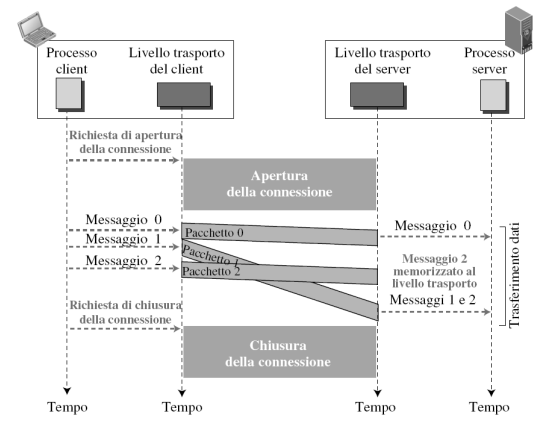
\includegraphics[width=9cm]{images/orient-conn.PNG}
    \caption{Servizi orientati alla connessione}
    \label{fig:orient-conn}
\end{figure}

A livello trasporto il servizio orientato alla connessione coinvolge solamente i due host finali: si tratta di un servizio end-to-end (tra le due estremità). Questo significa che dovrebbe essere possibile utilizzare un protocollo orientato alla connessione a livello trasporto indipendentemente dal protocollo di livello rete (con o senza connessione). In un protocollo orientato alla connessione è possibile implementare il controllo di flusso, il controllo degli errori e il controllo della congestione.

\subsubsection*{Rappresentazione tramite FSM}
Il comportamento di un protocollo del livello trasporto può essere ben rappresentato con una macchina o automa a stati finiti (FSM, Finite State Machine). La FSM di un livello trasporto orientato alla connessione deve passare attraverso tre stati prima di raggiungere lo stato established. La macchina è nello stato closed (chiuso) quando non vi è connessione e rimane in questo stato fino a quando arriva una richiesta di apertura della connessione dal processo locale: la macchina invia un pacchetto di richiesta di apertura al livello trasporto remoto e si sposta allo stato open-wait-I (attesa di apertura I). La FSM locale, quando riceve il riscontro dall'altro lato, si sposta allo stato open-wait-II (attesa di apertura II). Quando la macchina è in questo stato, è stata completata l'apertura di una connessione unidirezionale; se è richiesta una connessione bidirezionale, la macchina deve rimanere in attesa in questo stato fino a quando anche l'altro lato richiede l'apertura della connessione. Quando riceve la richiesta, la macchina invia un riscontro e passa allo stato established. I due lati possono scambiarsi dati e relativi riscontri mentre sono entrambi nello stato established.

Per chiudere una connessione, il livello applicazione invia un messaggio di richiesta di chiusura al proprio livello trasporto. Questo invia un pacchetto di richiesta di chiusura all'altro lato e si sposta nello stato close-wait-I. Quando riceve un riscontro dall'altro lato, la macchina si sposta nello stato close-wait-II dove attende il pacchetto con la richiesta di chiusura dall'altro lato. All'arrivo del pacchetto la macchina invia un riscontro e si sposta nello stato closed.

\begin{figure}[ht]
    \centering
    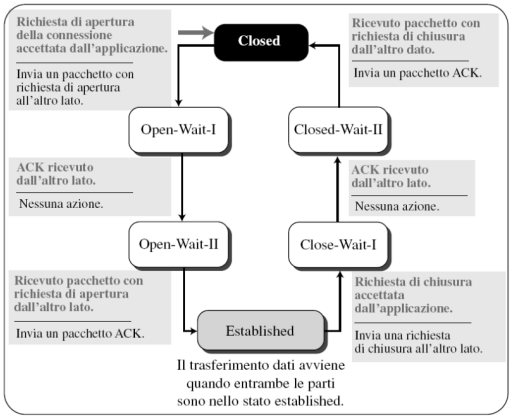
\includegraphics[width=9cm]{images/fsm-tcp.PNG}
    \caption{FSM per il livello trasporto orientato alla connessione}
    \label{fig:fsm-tcp}
\end{figure}

\subsubsection*{Controllo di flusso}
Quando un'entità produce dati che un'altra entità deve consumare, deve esistere un equilibrio fra la velocità di produzione e la velocità di consumo dei dati. Se i dati vengono prodotti a una velocità superiore rispetto a quella con cui possono essere consumati, il consumatore potrebbe trovarsi sovraccaricato ed essere costretto a eliminarne alcuni. Se i dati vengono prodotti a una velocità inferiore rispetto a quella con cui possono essere consumati, il consumatore deve rimanere in attesa, riducendo l'efficienza del sistema. Il controllo di flusso è legato alla prima problematica, dove si rende necessario evitare la perdita di dati al destinatario.

Nella comunicazione al livello trasporto si ha a che fare con quattro entità: il processo mittente, il livello trasporto del mittente, il livello trasporto del destinatario e il processo destinatario. Il processo mittente a livello applicazione è solo un produttore: produce dei dati e li passa al livello trasporto. Il livello trasporto del mittente ha un doppio ruolo: di consumatore e di produttore. Consuma i messaggi in arrivo dal produttore, li incapsula in pacchetti e li trasmette al livello trasporto del destinatario. Anche il livello trasporto del destinatario ha un doppio ruolo: è consumatore dei pacchetti in arrivo dal mittente ed è il produttore che decapsula i messaggi e li consegna al livello applicazione. L'ultima consegna, tuttavia, agisce solitamente in pulling: il livello trasporto attende fino a quando il processo di livello applicazione richiede dati. Sono necessari almeno due casi di controllo di flusso: dal livello trasporto al livello applicazione dal lato mittente, e dal livello trasporto del destinatario al livello trasporto del mittente.

\begin{figure}[ht]
    \centering
    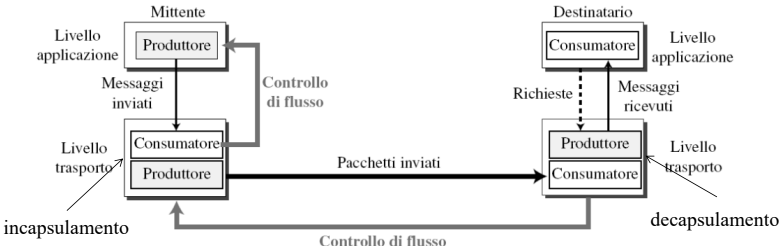
\includegraphics[width=11cm]{images/cont-flusso-tcp.PNG}
    \caption{Controllo del flusso al livello trasporto}
    \label{fig:cont-flusso-tcp}
\end{figure}

Sebbene il controllo di flusso possa essere realizzato in modi differenti, una delle soluzioni classiche consiste nell'utilizzare due buffer: uno al livello trasporto del mittente e l'altro al livello trasporto del destinatario. Un buffer è un insieme di locazioni di memoria che possono contenere dei pacchetti. La comunicazione delle informazioni di controllo di flusso può avvenire inviando segnali dal consumatore al produttore.

Il livello trasporto del mittente segnala al livello applicazione, quando ha il buffer saturo, di sospendere l'invio di messaggi; quando si libera dello spazio nel buffer segnala al livello applicazione che può riprendere l'invio di messaggi.

\subsubsection*{Controllo degli errori}
In Internet, dato che il livello rete (IP) è inaffidabile, è necessario implementare l'affidabilità al livello trasporto se richiesta dall'applicazione. L'affidabilità può essere ottenuta aggiungendo i servizi di controllo degli errori al livello trasporto, che ha la responsabilità di:
\begin{itemize}
    \item rilevare e scartare i pacchetti corrotti;
    \item tenere traccia dei pacchetti persi e scartati e gestirne la rispedizione;
    \item riconoscere i pacchetti duplicati ed eliminarli;
    \item bufferizzare i pacchetti fuori sequenza fino a quando arrivano i pacchetti mancanti.
\end{itemize}

Il controllo degli errori, a differenza del controllo di flusso, coinvolge solamente i livelli trasporto del mittente e del destinatario. Si suppone infatti che i messaggi scambiati fra i livelli applicazione siano esenti da errori. Il livello trasporto del destinatario gestisce il controllo degli errori, nella maggior parte dei casi, segnalando il problema al livello trasporto del mittente.

\begin{figure}[ht]
    \centering
    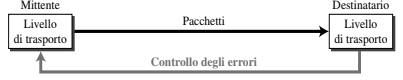
\includegraphics[width=9cm]{images/cont-err-tcp.PNG}
    \caption{Controllo degli errori al livello trasporto}
    \label{fig:cont-err-tcp}
\end{figure}

Il controllo degli errori comporta che il livello trasporto del mittente sappia quale pacchetto debba rispedire e che il livello trasporto del destinatario sappia riconoscere i pacchetti duplicati o fuori sequenza. Questo può essere ottenuto numerando i pacchetti, ovvero aggiungendo ai pacchetti del livello trasporto un campo che indica il loro numero di sequenza. Quando un pacchetto viene corrotto o smarrito, il livello trasporto del destinatario può chiedere al livello trasporto del mittente di rispedirlo, identificandolo tramite il numero di sequenza. Il livello trasporto del ricevente può identificare anche i pacchetti duplicati, quando riceve due pacchetti con il medesimo numero di sequenza. I pacchetti fuori sequenza possono infine essere identificati verificando gli eventuali numeri di sequenza ricevuti disordinatamente.

I pacchetti vengono numerati sequenzialmente. Tuttavia, poiché è necessario inserire il numero di sequenza nell'intestazione di ogni pacchetto, occorre specificarne il valore massimo. Se l'intestazione del pacchetto prevede di allocare $m$ bit per i numeri di sequenza, questi possono assumere i valori da $0$ a $2^m-1$. Se $m$ vale 4, per esempio, si possono utilizzare i numeri di sequenza da 0 a 15. Naturalmente, raggiunto l'ultimo numero si può ricominciare dal primo. I numeri di sequenza utilizzati per il controllo degli errori sono considerati in modulo $2^m$ dove $m$ è la dimensione del campo numero di sequenza espressa in bit.

Per notificare al mittente la corretta ricezione di uno o più pacchetti viene utilizzato il numero di riscontro (detto anche acknowledgment, ACK, o conferma). Il destinatario può semplicemente scartare (ignoras) i pacchetti corrotti. Il mittente può identificare i pacchetti persi utilizzando un timer. Quando invia un pacchetto, il mittente attiva un timer: se non riceve un ACK prima della sua scadenza rispedisce il pacchetto. Anche i pacchetti duplicati possono essere semplicemente scartati dal destinatario. I pacchetti fuori sequenza possono invece essere scartati (saranno trattati dal mittente come pacchetti persi) oppure temporaneamente memorizzati in attesa dell'arrivo dei pacchetti mancanti.

\subsubsection*{Integrazione del controllo degli errori e controllo di flusso}
Si è visto che il controllo di flusso richiede l'impiego di due buffer, uno nel mittente e l'altro nel destinatario. Si è visto anche che il controllo degli errori richiede l'uso dei numeri di sequenza e di riscontri in entrambi i lati. Questi due requisiti possono essere combinati usando due buffer numerati, uno presso il mittente e uno presso il destinatario.

Nel mittente, quando si prepara un pacchetto si usa il numero della posizione libera successiva nel buffer, $x$, come numero di sequenza del pacchetto. Quando il pacchetto viene inviato, ne viene memorizzata una copia nella locazione $x$, in attesa della sua conferma da parte del destinatario. Quando si riceve una conferma relativa a un pacchetto inviato, il pacchetto memorizzato viene climinato liberando la posizione di memoria che occupava. Un pacchetto con numero di sequenza $y$ che arriva al destinatario, viene memorizzato nella locazione $y$ fino a quando il livello applicazione è pronto a riceverlo. A quel punto può essere inviata la conferma di ricezione del pacchetto $y$.

Poiché il numero di sequenza è calcolato in modulo $2^m$, i numeri di sequenza da 0 a $2^m-1$ possono essere rappresentati con un cerchio. Il buffer viene rappresentato come un insieme di settori, chiamati finestra scorrevole (sliding window), che in ogni istante occupano una parte del cerchio. Nel mittente, quando viene inviato un pacchetto se ne contrassegna il settore corrispondente. Quando tutti i settori risultano contrassegnati, il buffer è completo e non possono essere accettati altri messaggi dal livello applicazione. Quando arriva un riscontro, viene eliminato il contrassegno dal settore corrispondente. Quando un insieme consecutivo di settori a partire dall'inizio della finestra risulta non contrassegnato, la finestra scorre sopra l'intervallo dei numeri di sequenza corrispondenti rendendo disponibile un numero di settori equivalente alla fine della finestra.

\begin{figure}[ht]
    \centering
    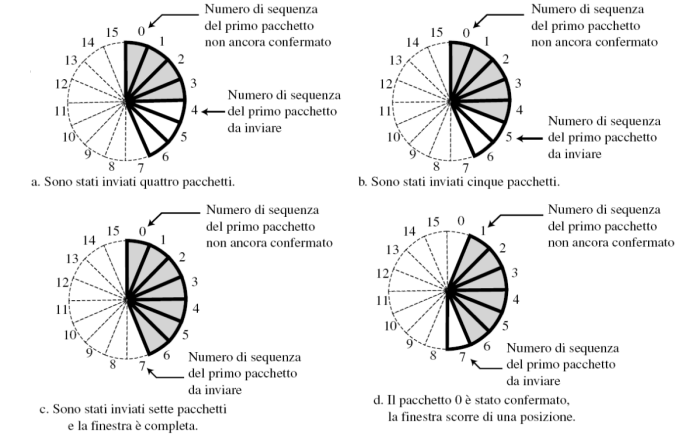
\includegraphics[width=11cm]{images/sliding-window.PNG}
    \caption{Finestra scorrevole con rappresentazione circolare}
    \label{fig:sliding-window}
\end{figure}

Si noti che la finestra scorrevole è solo un'astrazione: nella realtà si utilizzano delle variabili per contenere i numeri di sequenza del pacchetto successivo da inviare e dell'ultimo pacchetto inviato.

La maggior parte delle descrizioni dei protocolli rappresentano la finestra scorrevole con una rappresentazione lineare. L'idea è la stessa, ma la rappresentazione risultante è solitamente più sintetica.

\begin{figure}[ht]
    \centering
    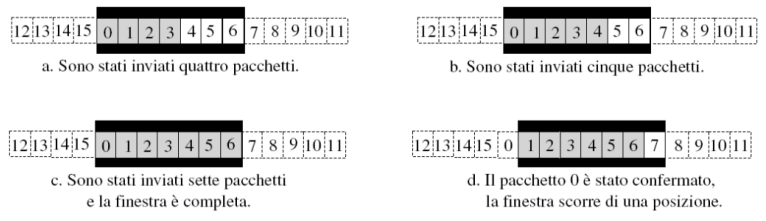
\includegraphics[width=11cm]{images/sliding-window2.PNG}
    \caption{Finestra scorrevole con rappresentazione lineare}
    \label{fig:sliding-window2}
\end{figure}

\subsubsection*{Controllo della congestione}
La congestione in una rete può avvenire se il carico della rete - il numero di pacchetti inviati alla rete - è superiore alla capacità della rete - il numero di pacchetti che una rete può gestire. L'espressione controllo della congestione fa riferimento ai meccanismi e alle tecniche per controllare la congestione mantenendo il carico della rete al di sotto della sua capacità.

Ci si potrebbe chiedere per quale motivo esista la congestione in una rete: la congestione può avvenire in qualsiasi sistema che comporti un'attesa. La congestione in rete può avvenire poiché i router e gli switch hanno delle code - buffer dove vengono memorizzati i pacchetti prima e dopo la loro elaborazione. Un router, per esempio, ha una coda di input e una coda di output per ogni interfaccia. Se il router non riesce a elaborare i pacchetti alla stessa velocità con cui arrivano, le code si sovraccaricano e avviene la congestione. La congestione a livello trasporto è in realtà il risultato della congestione a livello rete che si manifesta a livello trasporto.

\subsection{Stop-and-wait}
Il secondo meccanismo preso in considerazione è orientato alla connessione ed è chiamato Stop and Wait; utilizza sia il controllo di flusso sia il controllo degli errori. Il mittente e il destinatario usano entrambi una finestra scorrevole di dimensione 1. Il mittente invia un pacchetto alla volta e ne attende l'ack (riscontro) prima di poter spedire il successivo. Per rilevare i pacchetti corrotti è necessario aggiungere un valore checksum (valore di controllo) a ogni pacchetto dati. Quando un pacchetto arriva al destinatario, viene calcolato il checksum: se il valore corrisponde al checksum ricevuto, si invia un ack al mittente. Se il ckecksum non corrisponde, il pacchetto risulta corrotto e viene scartato senza informare il client. L'assenza di un ack da parte del destinatario costituisce un'indicazione per il mittente che il pacchetto è stato perso o scartato. Infatti, ogni volta che il mittente invia un pacchetto, inizializza un timer. Se arriva un ack prima che il timer sia scaduto, il timer viene arrestato e viene inviato il pacchetto successivo (se esiste un pacchetto pronto). Se invece il timer scade, il mittente rispedisce il pacchetto precedente, ipotizzando che sia stato corrotto o si sia smarrito. Questo comporta che il mittente deve tenere una copia del pacchetto fino a quando non ne riceve il riscontro. Si noti che in un dato istante, nel canale possono esserci un solo pacchetto e un solo riscontro.

\begin{figure}[ht]
    \centering
    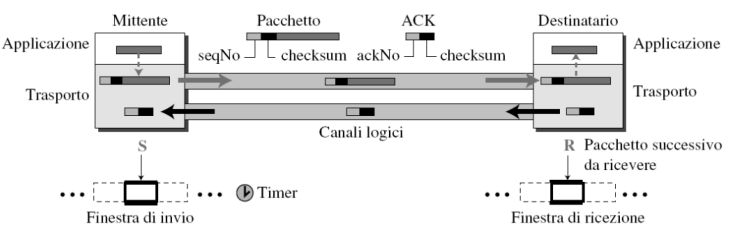
\includegraphics[width=12cm]{images/stop-and-wait.PNG}
    \caption{Stop and Wait}
    \label{fig:stop-and-wait}
\end{figure}

Il meccanismo Stop and Wait è orientato alla connessione e fornisce i servizi di controllo degli errori e del flusso (il controllo di flusso è garantito dal fatto che non si spedisce più di un pacchetto alla volta).

\subsubsection*{Numeri di sequenza e di riscontro}
Per poter gestire i pacchetti duplicati, lo Stop and Wait utilizza i numeri di sequenza e di riscontro. Viene quindi aggiunto un campo all'intestazione del pacchetto, per contenere il valore del numero di sequenza del pacchetto. Una considerazione importante riguarda l'intervallo dei possibili valori dei numeri di sequenza: l'obiettivo è sempre minimizzare la dimensione dei pacchetti, o meglio delle informazioni di controllo nei pacchetti. Si vuole quindi identificare l'intervallo più piccolo possibile che possa consentire la comunicazione senza ambiguità. Ebbene: se si è utilizzato $x$ come numero di sequenza, dopo di questo è sufficiente utilizzare il numero $x+1$, mentre il numero $x+2$ non è necessario. Per dimostrare questa affermazione, si supponga che il mittente abbia inviato il pacchetto con numero di sequenza $x$. Si possono verificare tre casi.
\begin{enumerate}
    \item Il pacchetto arriva correttamente al destinatario, che invia un riscontro. Il riscontro arriva al mittente, che invia il pacchetto successivo numerato $x+1$.
    \item Il pacchetto risulta corrotto o non arriva al destinatario. In questo caso il mittente, scaduto il timeout, rispedisce il pacchetto con numero di sequenza $x$, che viene normalmente riscontrato dal destinatario.
    \item Il pacchetto arriva correttamente al destinatario, ma il riscontro del destinatario viene perso o risulta corrotto. Il mittente rispedisce quindi il pacchetto (con numero di sequenza $x$) dopo il timeout. In questo caso il pacchetto ricevuto è un duplicato, ma il destinatario se ne accorge perché aspettandosi il pacchetto $x+1$ riceve il pacchetto $x$.
\end{enumerate}

Si può quindi osservare che i numeri di sequenza $x$ e $x+1$ sono necessari per disambiguare i casi 1 e 3, ma non vi è alcuna necessità del numero di sequenza $x+2$. Nel caso 1 il pacchetto può essere numerato nuovamente con $x$, poiché i pacchetti $x$ e $x+1$ sono già stati riscontrati e non vi possono essere ambiguità nei due siti. Nei casi 2 e 3 il nuovo pacchetto è $x+1$ non $x+2$. Se sono necessari solo $x$ e $x+1$, è possibile allora porre $x=0$ e $x+1=1$: in questo caso la sequenza sarà 0, 1, 0, 1, 0 e così via (aritmetica modulo 2).

Poiché i numeri di sequenza devono essere adatti sia per numerare i pacchetti dati sia per indicare i riscontri, si utilizza la seguente convenzione: il numero di riscontro indica sempre il numero di sequenza del prossimo pacchetto atteso dal destinatario. Se per esempio il destinatario ha ricevuto correttamente il pacchetto 0, invia un riscontro con valore 1 (che significa che il prossimo pacchetto atteso è quello con numero di sequenza 1). Se il destinatario ha ricevuto correttamente il pacchetto 1, invia il riscontro 0 (che significa che si attende il pacchetto 0).

Nel meccanismo Stop and Wait il numero di riscontro indica, in aritmetica modulo 2, il numero di sequenza del prossimo pacchetto atteso dal destinatario.

\subsubsection*{FSM}
Viene illustrato le FSM per il meccanismo Stop and Wait. Essendo orientato alla connessione, entrambi i lati devono essere nello stato established prima di poter trasmettere pacchetti dati. Gli stati indicati sono in realtà nidificati nello stato established. Il mittente è inizialmente nello stato ready (pronto), ma si può muovere fra gli stati ready e blocking (bloccato). La variabile $S$ viene inizializzata a 0.
\begin{itemize}
    \item \textit{Stato ready.} Il mittente in questo stato è in attesa di qualche evento. Se arriva una richiesta dal livello applicazione, crea un pacchetto con numero di sequenza $S$, memorizza una copia del pacchetto, lo invia, inizializza il timer e passa nello stato blocking.
    \item \textit{Stato blocking.} Quando il mittente è in questo stato possono avvenire tre eventi.
    \begin{enumerate}
        \item Se arriva un ACK integro (senza errori) con \verb|ackNo| (numero di riscontro) uguale al prossimo pacchetto da inviare, ovvero con $\verb|ackNo| = (S +1) \mod 2$, il timer viene interrotto, la finestra viene fatta scorrere in avanti calcolando $S = (S + 1) \mod 2$ e il mittente passa nello stato ready.
        \item Se viene ricevuto un ACK corrotto o integro ma con $\verb|ackNo|\neq (S + 1) \mod 2$, esso viene scartato.
        \item Se interviene un time-out (scade il timer), il mittente invia l'unico pacchetto ancora in sospeso (ancora non confermato) e fa ripartire il timer.
    \end{enumerate}
\end{itemize}

Il destinatario rimane sempre nello stato ready, dove possono avvenire tre eventi.
\begin{enumerate}
    \item Se arriva un pacchetto integro con $seqNo = R$, il messaggio nel pacchetto viene consegnato al livello applicazione, la finestra viene fatta scorrere calcolando $R = (R + 1) \mod 2$ e viene inviato un riscontro con $\verb|ackNo| = R$.
    \item Se arriva un pacchetto integro con $seqNo\neq R$, il pacchetto viene scartato ma viene inviato un riscontro con $\verb|ackNo| = R$.
    \item Se arriva un pacchetto corrotto, viene scartato.
\end{enumerate}

\begin{figure}[ht]
    \centering
    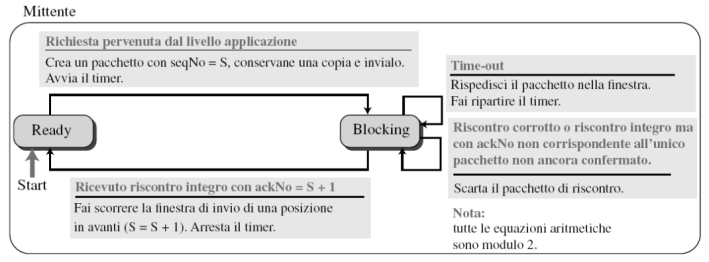
\includegraphics[width=11cm]{images/fsm-mitt-stop-and-wait.PNG}
    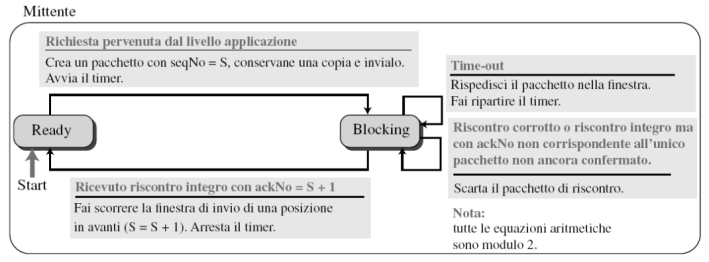
\includegraphics[width=11cm]{images/fsm-mitt-stop-and-wait.PNG}
    \caption{FSM per il mittente e destinatario Stop and Wait}
    \label{fig:mitt-dest-stop-and-wait}
\end{figure}

\subsubsection*{Efficienza}
Il meccanismo Stop and Wait è molto inefficiente se il canale è ha una velocità di trasmissione elevata (una banda passante elevata) e un lungo ritardo (tempo di andata e ritorno). Il prodotto di questi due valori è chiamato prodotto banda-ritardo.

\begin{Example}{Efficienza di Stop and Wait}{}
    \textit{In un sistema che utilizza un meccanismo Stop and Wait, l'ampiezza di banda del canale è di 1 Mbps; il tempo necessario a 1 bit per fare un viaggio di andata e ritorno è di 20 millisecondi. Quanto vale il prodotto banda-ritardo? Se i pacchetti dati del sistema hanno dimensione di 1000 bit, qual è la percentuale di utilizzo del canale?}

    Il prodotto banda-ritardo è pari a $(1x10^6)*(20x10^{-3}) = 20000 bit$. Il sistema potrebbe inviare 20000 bit nel tempo necessario ai dati per andare dal mittente al ricevente e per ottenerne il riscontro, tuttavia invia solamente 1000 bit. Si può affermare che il coefficiente di utilizzo del canale è solamente di 1000/20000, ovvero del 5\%. Per questo motivo l'impiego del meccanismo Stop and Wait in un canale con elevato ritardo o con elevata velocità è inefficiente.
\end{Example}

\subsection{Go-Back-N (GBN)}
Nel meccanismo di Stop and Wait il mittente deve attendere che il pacchetto precedente abbia raggiunto il destinatario e che il relativo riscontro sia stato ricevuto, prima di poter inviare il pacchetto successivo.

Tuttavia, per migliorare l'efficienza di trasmissione si devono avere più pacchetti in transizione mentre il mittente è in attesa dei riscontri. Ovvero è necessario consentire di lasciare in sospeso (in attesa di riscontro) più di un pacchetto, mantenendo il canale occupato mentre il mittente è in attesa dei riscontri. Un primo meccanismo che consente di raggiungere questo obiettivo, è chiamato Go-Back-N (GBN) (riparti da N). Questo meccanismo adotta la tecnica del pipeling, ovvero permette di inviare più pacchetti senza dover attendere il riscontro ai primi pacchetti inviati.

Il concetto alla base del Go-Back-N è proprio la possibilità di inviare diversi pacchetti prima di ricevere dei riscontri, ma il destinatario può bufferizzare un solo pacchetto. Il mittente mantiene una copia dei pacchetti inviati fino a quando non ne riceve un riscontro. Si noti che più pacchetti dati e i relativi riscontri possono essere contemporaneamente nel canale.

\begin{figure}[ht]
    \centering
    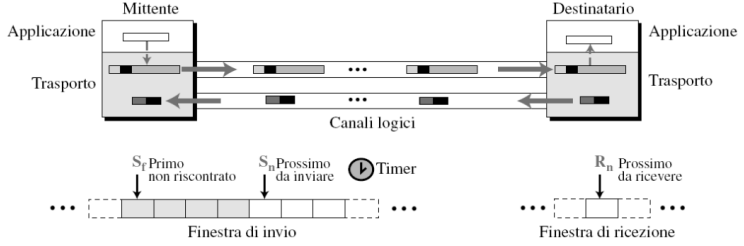
\includegraphics[width=12cm]{images/go-back-n.PNG}
    \caption{Schema generale del meccanismo Go-Back-N}
    \label{fig:go-back-n}
\end{figure}

\subsubsection*{Numeri di sequenza e di riscontro}
In Go-Back-N i numeri di sequenza sono calcolati modulo $2^m$, dove $m$ è la dimensione del campo sequence number in bit.

Il numero di riscontro in questo caso è cumulativo e indica il numero di sequenza del prossimo pacchetto atteso. Per esempio, se il numero di riscontro (\verb|ackNo|) vale 7 significa che tutti i pacchetti fino al 6 sono stati ricevuti correttamente e che il destinatario si attende di ricevere il pacchetto con numero di sequenza 7.

\subsubsection*{Finestra di invio}
La finestra di invio è una scatola immaginaria che ricopre i numeri di sequenza dei pacchetti che possono essere in transito o che possono essere spediti. Per ciascuna posizione di questa finestra, alcuni dei numeri di sequenza corrispondono ai pacchetti inviati, altri corrispondono a quelli che possono essere inviati. La dimensione massima della finestra è $2^m-1$.

\begin{figure}[ht]
    \centering
    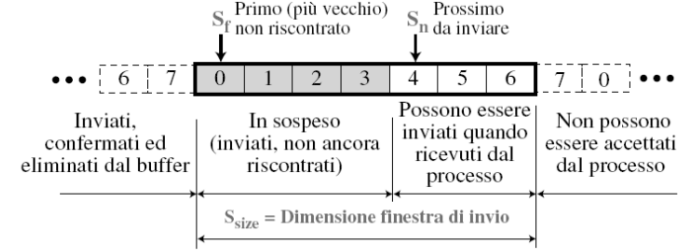
\includegraphics[width=10cm]{images/finestra-invio.PNG}
    \caption{Finestra di invio per il meccanismo Go-Back-N}
    \label{fig:finestra-invio}
\end{figure}

La finestra di invio in ogni istante divide i possibili numeri di sequenza in quattro regioni. La prima, alla sinistra della finestra, corrisponde ai numeri di sequenza dei pacchetti già confermati. Il mittente non si preoccupa di questi pacchetti e non ne mantiene copia. La seconda regione, su sfondo grigio, definisce l'intervallo dei numeri di sequenza dei pacchetti che sono stati inviati ma con stato ancora ignoto. Il mittente deve attendere per scoprire se sono stali ricevuti correttamente o se si sono persi; possono essere chiamati pacchetti in sospeso, o in attesa di riscontro. Il terzo intervallo, bianco nella figura, definisce l'intervallo dei numeri di sequenza dei pacchetti che possono essere inviati; tuttavia i dati corrispondenti non sono ancora stati ricevuti dal livello applicazione. Infine la quarta regione, alla destra della finestra, definisce i numeri di sequenza che non possono essere utilizzati fino a quando la finestra non avanza.

La finestra è ovviamente un concetto astratto: tre variabili ne definiscono le dimensioni e la posizione in ogni istante. Le variabili sono: $S_f$, (da Send First) ovvero primo pacchetto in attesa di riscontro nella finestra di invio, $S_n$ (da Send Next) ovvero prossimo pacchetto da inviare nella finestra di invio, e $S_{size}$ (da Send Size) ovvero dimensione della finestra di invio. La variabile $S_f$ definisce il numero di sequenza del primo (il più vecchio) pacchetto in attesa di riscontro. La variabile $S_n$ definisce il numero di sequenza che verrà assegnato al prossimo pacchetto da inviare. $S_{size}$ definisce la dimensione della finestra, che si suppone fissa nel protocollo in esame.

\begin{figure}[ht]
    \centering
    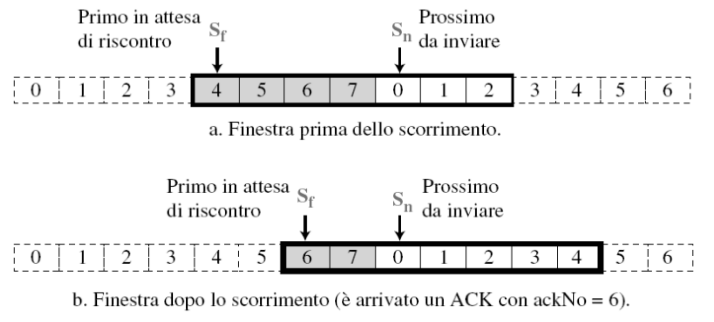
\includegraphics[width=10cm]{images/es-finestra-scorr.PNG}
    \caption{Scorrimento della finestra di invio}
    \label{fig:es-finestra-scorr}
\end{figure}

La finestra di invio può scorrere una o più posizioni quando viene ricevuto un riscontro privo di errori con \verb|ackNo| maggiore o uguale a $S_f$ e minore di $S_n$ (in aritmetica modulare).

\subsubsection*{Finestra di ricezione}
La finestra di ricezione permette di ricevere i pacchetti dati corretti e inviare i relativi riscontri. Nel meccanismo Go-Back-N, la dimensione della finestra di ricezione è sempre 1. Il destinatario è sempre in attesa dell'arrivo di un pacchetto specifico. Qualsiasi pacchetto arrivato fuori sequenza viene scartato e deve essere rispedito. Si noti che per definire lo stato della finestra è necessaria una sola variabile, $R_n$, (da Receive Next) ovvero prossimo pacchetto atteso nella finestra di ricezione. I numeri di sequenza alla sinistra della finestra appartengono ai pacchetti già ricevuti e riscontrati; i numeri di sequenza alla destra della finestra indicano i pacchetti che non possono ancora essere ricevuti. Qualsiasi pacchetto ricevuto in queste due regioni viene scartato. Viene accettato e riscontrato solo il pacchetto con numero di sequenza uguale a $R_n$. Anche la finestra di ricezione scorre, ma di una sola posizione. Quando viene ricevuto un pacchetto corretto, la finestra scorre: $R_n = (R_n + 1) \mod 2^m$.

\begin{figure}[ht]
    \centering
    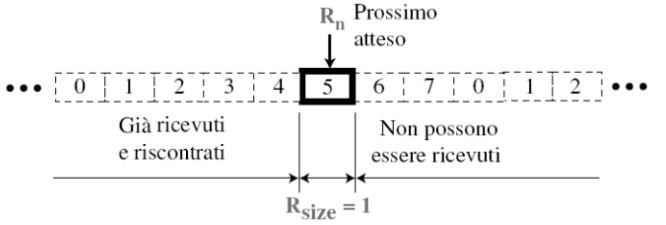
\includegraphics[width=9cm]{images/finestra-recezione-gbn.JPG}
    \caption{Finestra di recezione per il meccanismo Go-Back-N}
    \label{fig:es-finestra-scorr}
\end{figure}

\subsubsection*{Timer e rispedizione dei pacchetti}
Sebbene vi possa essere un timer per ciascun pacchetto inviato, nel meccanismo in esame se ne usa uno solo. Il motivo è dovuto al fatto che il timer del primo pacchetto in attesa di riscontro scade sempre per primo. Quando questo timer scade, si rispediscono tutti i pacchetti in attesa di riscontro.

Per esempio, si supponga che il mittente abbia già inviato il pacchetto $6 (S_n = 7)$ e che scada l'unico timer. Se $S_f = 3$ significa che i pacchetti 3, 4, 5 e 6 non sono stati riscontrati; il mittente torna indietro e rispedisce i pacchetti 3, 4, 5 e 6. Questo è il motivo per cui questo meccanismo viene chiamato Go-Back-N: allo scadere di un timeout la macchina torna indietro di N posizioni e rispedisce tutti i pacchetti.

\subsubsection*{FSM}
Il mittente inizia nello stato ready ma può successivamente trovarsi in due stati: ready o blocking. Le due variabili sono solitamente inizializzate a 0 ($S_f= S_n = 0$).
\begin{itemize}
    \item \textit{Stato ready.} Quando il mittente è in questo stato, possono avvenire quattro eventi.
    \begin{enumerate}
        \item Se arriva una richiesta dal livello applicazione, il mittente crea un pacchetto con numero di sequenza impostato a $S_n$. Il pacchetto viene memorizzato e inviato. Il mittente avvia anche l'unico timer (se questo non fosse già stato attivato). Viene quindi incrementato il valore di $S_n: S_n = (S_n+1) \mod 2^m$. Se la finestra è tutta occupata, ovvero $S_n=(S_f+S_n) \mod 2^m$, il mittente si sposta nello stato bloccato.
        \item Se arriva un riscontro integro con \verb|ackNo| relativo a uno dei pacchetti in attesa di riscontro, il mittente fa scorrere la finestra (imposta $S_f$= \verb|ackNo|); se tutti i pacchetti in attesa di riscontro sono confermati (\verb|ackNo| = $S_n$) il timer viene interrotto; se c'è almeno un pacchetto in attesa di riscontro, il timer viene riavviato.
        \item Se viene ricevuto un riscontro corrotto o con \verb|ackNo| non corrispondente ad alcun pacchetto in attesa di riscontro, il riscontro viene scartato.
        \item Se avviene un timeout, il mittente rispedisce tutti i pacchetti in attesa di riscontro e riavvia il timer.
    \end{enumerate}
    \item \textit{Stato blocking.} In questo caso possono avvenire tre eventi.
    \begin{enumerate}
        \item Se arriva un riscontro integro con \verb|ackNo| corrispondente a uno dei pacchetti in attesa di riscontro, il mittente fa scorrere la finestra (imposta $S_f$ = \verb|ackNo|) e se tutti i pacchetti in attesa di riscontro sono confermati (\verb|ackNo| = $S_n$) il timer viene arrestato. Se non tutti i pacchetti in attesa di riscontro risultano confermati, viene riavviato il timer. Il mittente passa quindi allo stato ready.
        \item Se si riceve un pacchetto di conferma corrotto o con \verb|ackNo| non corrispondente ad alcun pacchetto in attesa di riscontro, la conferma viene scartata.
        \item Se avviene un timeout, il mittente rispedisce tutti i pacchetti in attesa di riscontro e riavvia il timer.
    \end{enumerate}
\end{itemize}

Il destinatario rimane sempre nello stato ready. L'unica variabile $R_n$, viene inizializzata a 0. Possono avvenire tre eventi.
\begin{enumerate}
    \item Se viene ricevuto un pacchetto integro con \verb|seqNo| = $R_n$, il messaggio contenuto nel pacchetto viene consegnato al livello applicazione e la finestra viene fatta scorrere: $R_n=(R_n+1) \mod 2^m$. Infine viene inviato un riscontro con \verb|ackNo| = $R_n$.
    \item Se viene ricevuto un pacchetto con \verb|seqNo| all'esterno della finestra, il pacchetto viene scartato e viene inviato un riscontro con \verb|ackNo| = $R_n$.
    \item Se viene ricevuto un pacchetto corrotto, viene semplicemente scartato.
\end{enumerate}

\begin{figure}[ht]
    \centering
    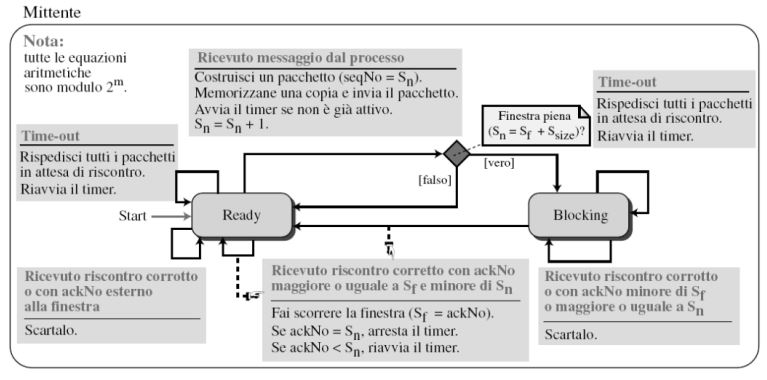
\includegraphics[width=0.5\textwidth]{images/mit-fsm-gbn.JPG}
    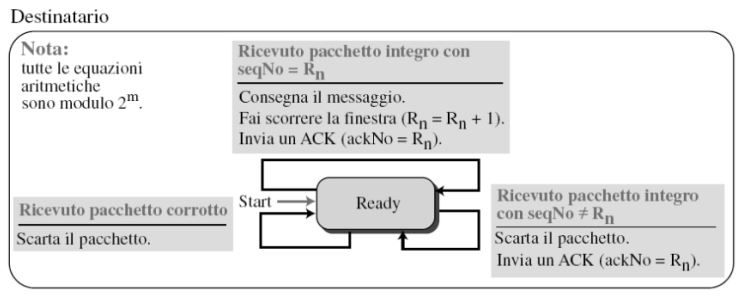
\includegraphics[width=0.49\textwidth]{images/dest-fsm-gbn.JPG}
    \caption{FMS per il meccanismo GBN}
    \label{fig:es-finestra-scorr}
\end{figure}

\begin{Example}{Go-Back-N in azione (ack cumulativo)}{}
    \textit{Viene illustrato ciò che avviene quando si perde un pacchetto.}

    \begin{minipage}[c]{0.55\textwidth}
        I pacchetti 0, 1, 2 e 3 vengono inviati ma viene smarrito il pacchetto 1. Il destinatario riceve i pacchetti 2 e 3, ma questi vengono scartati poiché ricevuti fuori sequenza (il pacchetto atteso è il numero 1). Quando il destinatario riceve i pacchetti 2 e 3, invia un riscontro ACK 1 per indicare che si attende il pacchetto 1. Questi riscontri non sono utili al mittente poiché l'\verb|ackNo| è uguale a $S_f$, non è strettamente maggiore di $S_f$; quindi vengono ignorati. Quando scade il timeout, il mittente rispedisce i pacchetti 1, 2 e 3, che vengono riscontrati.
    \end{minipage}
    \hfill
    \begin{minipage}[c]{0.44\textwidth}
        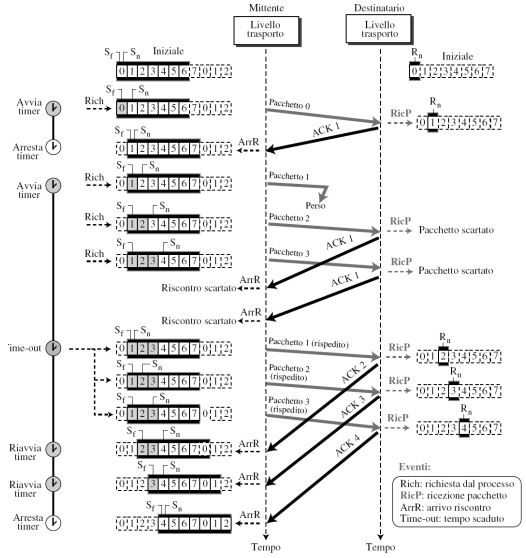
\includegraphics[width=1\textwidth]{images/es-flusso-gbn.JPG}
    \end{minipage}
\end{Example}

\subsubsection*{Dimensione della finestra di invio}
Si può ora dimostrare il motivo per cui la dimensione della finestra di invio deve essere inferiore a $2^m$. Si scelga per esempio $m = 2$, che significa che la dimensione della finestra può essere $2^m-1$, ovvero 3. Se la dimensione della finestra è 3 (minore di $2^m$) e tutti e tre i riscontri vengono persi, l'unico timer scade e vengono rispediti tutti e tre i pacchetti. Il destinatario si aspetta ora il pacchetto 3, non il pacchetto 0, così che il pacchetto duplicato viene correttamente scartato. Se invece la dimensione della finestra fosse 4 (ovvero uguale a $2^m$) e tutti i riscontri venissero persi, il mittente invierebbe un duplicato del pacchetto 0. Tuttavia questa volta la finestra del destinatario si aspetta di ricevere il pacchetto 0 (nel ciclo successivo), quindi accetta il pacchetto 0 non come duplicato, ma come primo pacchetto del nuovo ciclo. Evidentemente si tratta di un errore: questo dimostra che la dimensione della finestra di invio deve quindi essere inferiore a $2^m$.

\begin{figure}[ht]
    \centering
    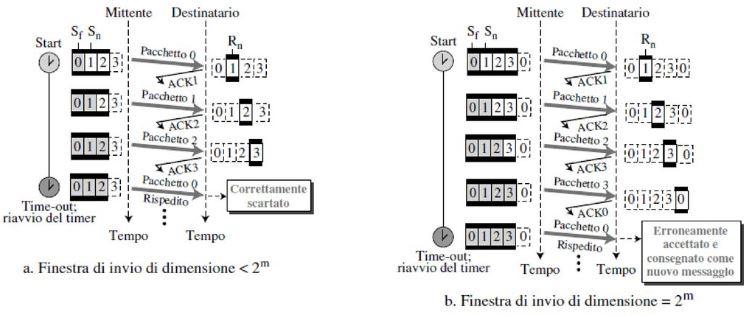
\includegraphics[width=14cm]{images/dim-finestra-invio-gbn.JPG}
    \caption{Dimensione della finestra di invio per Go-Back-N}
    \label{fig:es-finestra-scorr}
\end{figure}

Nel meccanismo Go-Back-N, la dimensione della finestra di invio deve essere inferiore a $2^m$; la dimensione della finestra di ricezione è sempre 1.

\subsection{Ripetizione selettiva}
Il meccanismo Go-Back-N semplifica i compiti del destinatario, che tiene traccia di una sola variabile e non deve bufferizzare i pacchetti fuori sequenza: questi vengono semplicemente ignorati. Questo meccanismo è tuttavia inefficiente se il livello rete sottostante perde numerosi pacchetti. Ogni volta che un singolo pacchetto risulta corrotto o smarrito, il mittente deve inviare tutti i pacchetti in attesa di riscontro anche se alcuni di questi sono già stati ricevuti correttamente ma fuori sequenza. Se il livello rete perde pacchetti in numero elevato a causa della congestione nella rete, la rispedizione di tutti i pacchetti in attesa di riscontro peggiora la congestione, che alla fine comporta la perdita di un numero ancora superiore di pacchetti, portando al collasso totale della rete.

E' stato sviluppato un altro meccanismo, chiamato Selective-Repeat (SR) o ripetizione selettiva, che, come indicato dal nome, rispedisce i pacchetti selettivamente, ovvero solo quelli che sono realmente stati smarriti.

\begin{figure}[ht]
    \centering
    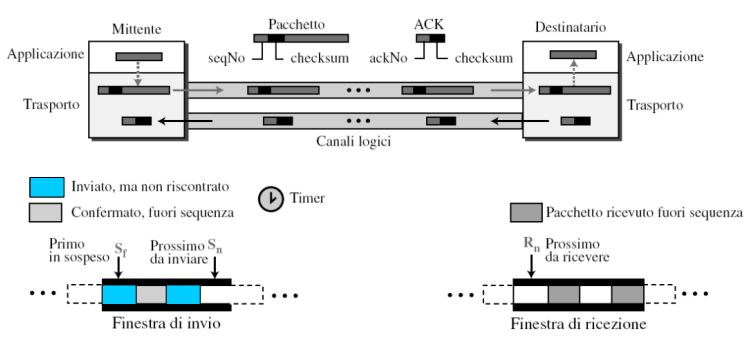
\includegraphics[width=11cm]{images/sr-schema-generale.JPG}
    \caption{Schema generale del meccanismo Selective-Repeat}
    \label{fig:es-finestra-scorr}
\end{figure}

\subsubsection*{Finestre di invio e recezione}
Anche il meccanismo Selective-Repeat utilizza due finestre: una di invio e l'altra di ricezione. Tuttavia vi sono delle differenze con le finestre del Go-Back-N. Per prima cosa la dimensione massima della finestra di invio è molto più piccola, $2^{m-1}$. Secondo, la dimensione della finestra di ricezione è uguale alla dimensione della finestra di invio. 

La dimensione massima della finestra di invio è $2^{m-1}$. Per esempio, se $m = 4$, i numeri di sequenza vanno da 0 a 15, ma la dimensione massima della finestra è 8 (mentre sarebbe 15 con il Go-Back-N). 

\begin{figure}[ht]
    \centering
    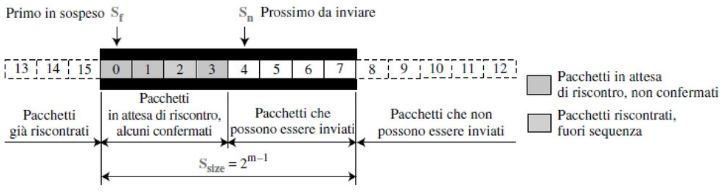
\includegraphics[width=11cm]{images/finestra-invio-sr.JPG}
    \caption{Finestra di invio del meccanismo Selective-Repeat}
    \label{fig:es-finestra-scorr}
\end{figure}

La finestra di ricezione nel Selective-Repeat è totalmente differente da quella nel Go-Back-N. La dimensione della finestra di ricezione è la stessa della finestra di invio (massimo $2^{m-1}$). Il meccanismo Selective-Repeat permette a un numero di pacchetti uguale alla dimensione della finestra di arrivare fuori sequenza; i pacchetti vengono memorizzati nella finestra fino a quando si forma un blocco di pacchetti consecutivi da passare al livello applicazione. Poiché la dimensione delle finestre di invio e di ricezione è la stessa, tutti i pacchetti nella finestra di invio possono arrivare fuori sequenza ed essere memorizzati fino a quando possono essere consegnati. Nella finestra, le celle ombreggiate indicano i pacchetti che sono arrivati fuori sequenza e che sono in attesa dell'arrivo dei pacchetti trasmessi in precedenza prima di poter essere passati al livello applicazione.

\begin{figure}[ht]
    \centering
    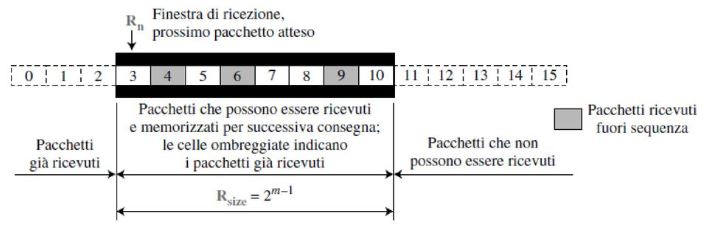
\includegraphics[width=11cm]{images/finestra-recezione-sr.JPG}
    \caption{Finestra di recezione del meccanismo Selective-Repeat}
    \label{fig:es-finestra-scorr}
\end{figure}

\subsubsection*{Timer}
Teoricamente il Selective-Repeat usa un timer per ciascun pacchetto in attesa di riscontro. Quando un timer scade ne viene rispedito solo il relativo pacchetto. A differenza di GBN che gestisce i pacchetti in attesa di riscontro come un singolo gruppo, SR li gestisce individualmente. La maggior parte dei protocolli di livello trasporto che implementano SR usa tuttavia un solo timer: per questo motivo anche in questo testo si usa un solo timer.

\subsubsection*{Riscontri}
Vi è un'ulteriore differenza fra i due meccanismi. Nel GBN il riscontro è cumulativo, indica il numero di sequenza del pacchetto successivo atteso, confermando che tutti i pacchetti precedenti sono stati ricevuti correttamente. La semantica dei riscontri in SR è invece differente: il numero di riscontro indica il numero di sequenza di un singolo pacchetto ricevuto correttamente, non può fornire feedback per gli altri.

Nel meccanismo Selective-Repcat il numero di riscontro indica il numero di sequenza di uno specifico pacchetto ricevuto senza errori.

\subsubsection*{FSM}
Le FSM per il meccanismo Selective-Repeat sono simili a quelle per GBN, ma vi sono delle differenze.

Il mittente inizia nello stato ready, ma successivamente può trovarsi negli stati ready o blocking. Ecco gli eventi e le azioni corrispondenti in ciascuno stato.

\begin{itemize}
    \item \textit{Stato ready.} In questo caso possono avvenire quattro eventi.
    \begin{enumerate}
        \item Se arriva una richiesta dal livello applicazione, il mittente crea un pacchetto con numero di sequenza impostato a $S_n$. Il pacchetto viene inviato dopo averne memorizzato una copia. Se il timer non è già attivo, viene inizializzato. Il valore di $S_n$, viene incrementato: $S_n = (S_n+1) \mod 2^m$. Se la finestra è completa, ovvero vale $S_n = (S_f+S_{size}) \mod 2^m$, il mittente passa nello stato blocked.
        \item Se viene ricevuto un riscontro integro con \verb|ackNo| relativo a uno dei pacchetti in attesa di riscontro, quel pacchetto viene contrassegnato come riscontrato. Se \verb|ackNo| = $S_f$ la finestra scorre a destra fino a quando $S_f$, punta al primo pacchetto non riscontrato (tutti i pacchetti consecutivi riscontrati sono ora all'esterno della finestra). Se vi sono ancora pacchetti in attesa di riscontro viene fatto ripartire il timer, altrimenti viene arrestato.
        \item Se viene ricevuto un riscontro corrotto o con \verb|ackNo| non relativo a uno dei pacchetti in attesa di riscontro, viene scartato.
        \item Se scade un timer, il mittente rispedisce tutti i pacchetti non confermati nella finestra e riavvia il timer.
    \end{enumerate}
    \item \textit{Stato blocking.} In questo caso possono avvenire tre eventi.
    \begin{enumerate}
        \item Se viene ricevuto un riscontro corretto con \verb|ackNo| relativo a uno dei pacchetti in attesa di riscontro, quel pacchetto viene contrassegnato come riscontrato. Inoltre, se \verb|ackNo| = $S_f$, la finestra viene fatta scorrere alla destra fino a che $S_f$, punta al primo pacchetto non riscontrato (tutti i pacchetti riscontrati consecutivi sono ora all'esterno della finestra). In questo ultimo caso il mittente passa nello stato ready.
        \item Se viene ricevuto un riscontro corrotto o con \verb|ackNo| non relativo a uno dei pacchetti in attesa di riscontro, il riscontro viene ignorato.
        \item Se scade un timer, il mittente rispedisce tutti i pacchetti non confermati nella finestra e riavvia il timer.
    \end{enumerate}
\end{itemize}

Il destinatario è sempre nello stato ready, nel quale possono avvenire tre eventi.
\begin{enumerate}
    \item Se viene ricevuto un pacchetto con \verb|seqNo| nella finestra, esso viene memorizzato e viene inviato un riscontro con \verb|ackNo| = \verb|seqNo|. Inoltre, se \verb|seqNo| = $R_n$, il pacchetto e tutti gli altri consecutivi arrivati in precedenza vengono passati al livello applicazione: la finestra viene fatta scorrere in modo che $R_n$, punti alla prima cella libera.
    \item Se viene ricevuto un pacchetto integro ma con \verb|seqNo| all'esterno della finestra, il pacchetto viene scartato ma viene inviato al mittente un riscontro con \verb|ackNo| = $R_n$. Questo è necessario per consentire al mittente di far scorrere la propria finestra nel caso qualche riscontro ai pacchetti con \verb|seqNo| $< R_n$, fosse andato perso.
    \item Se viene ricevuto un pacchetto corrotto, esso viene scartato.
\end{enumerate}

\begin{figure}[ht]
    \centering
    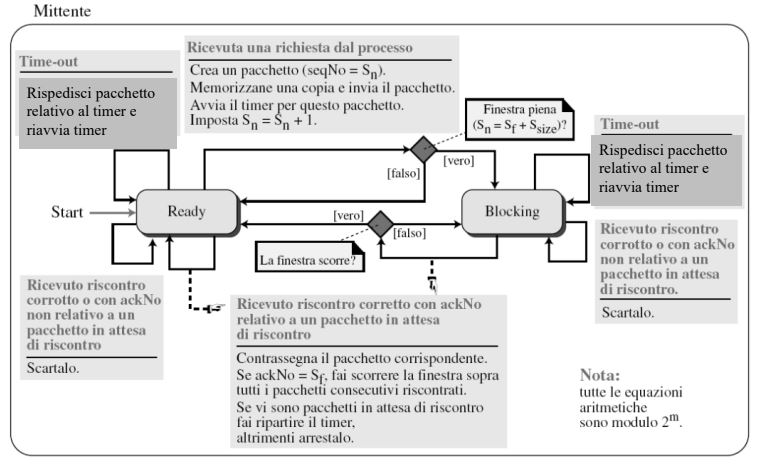
\includegraphics[width=0.50\textwidth]{images/mit-fsm-sr.JPG}
    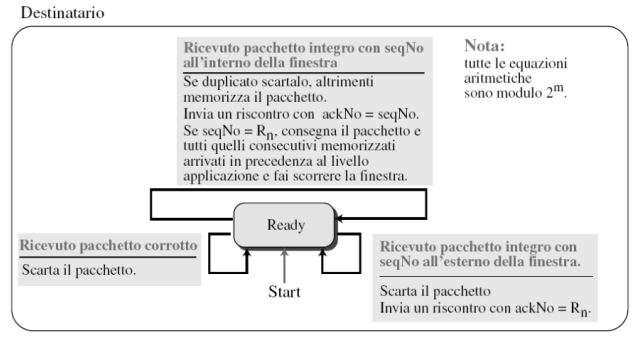
\includegraphics[width=0.49\textwidth]{images/dest-fsm-sr.JPG}
    \caption{FSM per il meccanismo Selective-Repeat}
    \label{fig:es-finestra-scorr}
\end{figure}

\begin{Example}{Selective-Repeat in azione}{}
    \textit{Viene illustrato il comportamento del Selective-Repeat.}

    \begin{minipage}{\textwidth}
        \centering
        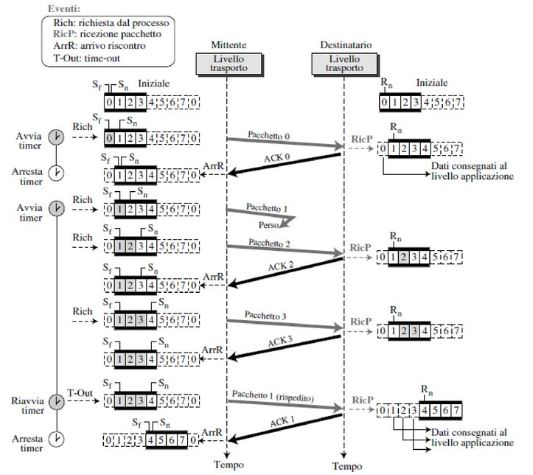
\includegraphics[width=0.6\textwidth]{images/es-flusso-sr.JPG}
        %\captionof{figure}{Esempio}
    \end{minipage}

    Il mittente trasmette il pacchetto 0 che viene riscontrato. Il pacchetto 1 viene perso, i pacchetti 2 e 3 arrivano fuori sequenza e vengono riscontrati. Quando scade il timer, il pacchetto 1 (l'unico non riscontrato) è rispedito e riscontrato. La finestra di invio viene fatta scorrere.

    Nel destinatario è necessario distinguere fra la ricezione di un pacchetto e la sua consegna al livello applicazione. Il pacchetto 2 viene ricevuto e memorizzato (cella ombreggiata), ma non può essere consegnato al livello applicazione poiché manca ancora il pacchetto 1. Successivamente arriva il pacchetto 3, che viene memorizzato: ancora non può essere consegnato alcun pacchetto poiché manca sempre il pacchetto 1. Solo quando finalmente viene ricevuta una copia del pacchetto 1, i pacchetti 1, 2 e 3 possono essere consegnati al livello applicazione.
\end{Example}

I pacchetti possono essere consegnati al livello applicazione se si verificano due condizioni. Per prima cosa deve essere stato ricevuto un insieme di pacchetti consecutivi. Secondo, l'insieme deve partire dall'inizio della finestra. Un livello trasporto affidabile consegna quindi i pacchetti secondo la sequenza di invio.

\subsubsection*{Dimensione delle finestre di invio e recezione}
E' ora possibile comprendere il motivo per cui la dimensione delle finestre di invio e di ricezione può essere al massimo la metà di $2^m$. Si scelga come esempio $m = 2$, che significa che la dimensione della finestra è $2^m/2$ ovvero $2^{(m-1)} = 2$.

Se la dimensione della finestra vale 2 e tutti i riscontri vengono persi, il timer del pacchetto 0 scade e il pacchetto viene quindi rispedito. Tuttavia la finestra del destinatario è in attesa del pacchetto 2, non del pacchetto 0 - quindi il pacchetto ricevuto viene correttamente scartato (il numero di sequenza 0 non è nella finestra). Quando la dimensione della finestra è 3 e tutti i riscontri vengono persi, il mittente invia un duplicato del pacchetto 0: questa volta la finestra del destinatario si aspetta di ricevere il pacchetto 0 (0 fa parte della finestra), quindi accetta questo pacchetto 0 non come duplicato, ma come se fosse un pacchetto del ciclo successivo. Evidentemente si tratta di un errore.

\begin{figure}[ht]
    \centering
    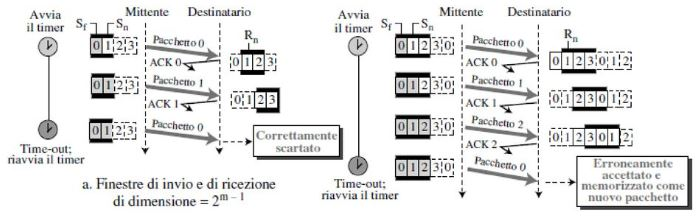
\includegraphics[width=13cm]{images/dim-finestra-invio-sr.JPG}
    \caption{Dimesione della finestra nel meccanismo Selective-Repeat}
    \label{fig:es-finestra-scorr}
\end{figure}

Nel meccanismo Selective-Repeat la dimensione delle finestre di invio e di ricezione può essere al massimo la metà di $2^m$.

\subsection{Protocolli bidirezionali: piggybacking}
I quattro meccanismi discussi in precedenza sono tutti unidirezionali: i pacchetti dati scorrono solo in una direzione e i riscontri nella direzione opposta. I pacchetti dati vengono in realtà trasmessi solitamente in entrambe le direzioni: dal client al server e dal server al client. Questo significa che anche i riscontri devono viaggiare in entrambe le direzioni. Per migliorare l'efficienza dei protocolli bidirezionali viene utilizzata una tecnica chiamata piggybacking ("viaggiare in spalla a qualcuno"). Quando un pacchetto trasporta dei dati da A a B, può trasportare anche i riscontri relativi ai pacchetti ricevuti da B; viceversa, quando un pacchetto trasporta dei dati da B ad A, può trasportare anche i riscontri relativi ai pacchetti ricevuti da A.

In questo sistema il client e il server usano entrambi due finestre indipendenti di invio e di ricezione.

\subsection{Segmenti TCP}
Sebbene la bufferizzazione possa gestire la differenza di velocità fra i processi produttore e consumatore, è necessario un passo ulteriore per poter trasmettere i dati. Il livello rete, quale fornitore di servizi al protocollo di livello trasporto (in questo caso TCP), deve inviare i dati in pacchetti, e non come flusso di byte. A livello trasporto, TCP raggruppa quindi un certo numero di byte in unità chiamate segmenti. TCP aggiunge un'intestazione formata da varie informazioni di controllo a ciascun segmento, che consegna al livello rete per la trasmissione. I segmenti vengono incapsulati in datagrammi IP e trasmessi. Tutte queste operazioni risultano essere perfettamente trasparenti al processo ricevente.

\begin{figure}[ht]
    \centering
    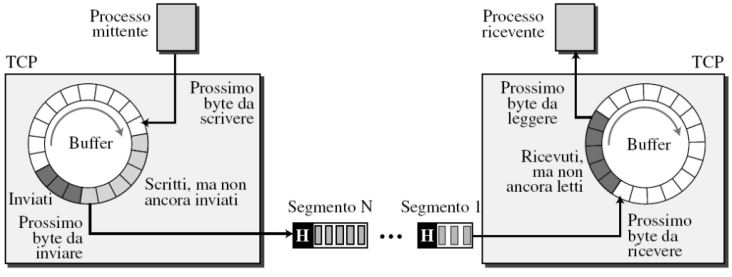
\includegraphics[width=10cm]{images/segmenti-tcp.JPG}
    \caption{Segmenti TCP}
    \label{fig:segmenti-tcp}
\end{figure}

Il segmento consiste di un'intestazione di dimensione compresa tra i 20 e i 60 byte, seguito dai dati provenienti dal programma applicativo. La dimensione dell'intestazione è di 20 byte in assenza di opzioni, fino a 60 byte altrimenti.

\begin{figure}[ht]
    \centering
    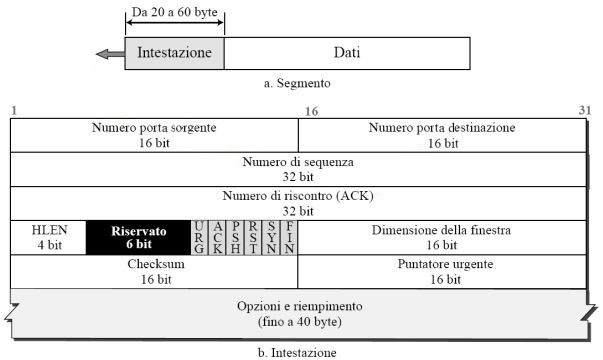
\includegraphics[width=10cm]{images/struttura-segmenti.JPG}
    \caption{Formato dei segmenti TCP}
    \label{fig:struttura-segmenti-tcp}
\end{figure}

\begin{itemize}
    \item \textit{Numero di porta sorgente.} Campo a sedici bit contenente il numero di porta del processo mittente sull'host che invia il segmento.
    \item \textit{Numero di porta destinazione.} Campo a sedici bit contenente il numero di porta del processo destinatario sull'host che riceve il segmento.
    \item \textit{Numero di sequenza.} Campo a 32 bit contenente il numero attribuito al primo byte di dati contenuto nel segmento. Più precisamente il numero di sequenza indica al destinatario quale dei byte inviati dal processo mittente è stato inserito come primo byte del segmento.
    \item \textit{Numero di riscontro (acknowledgement number).} Campo a 32 bit che contiene il numero di sequenza del byte che il destinatario si aspetta di ricevere. Per esempio se il destinatario ha ricevuto il byte con numero di sequenza $x$, restituirà il numero di riscontro pari a $x+1$.
    \item Lunghezza dell'intestazione (HLEN). Campo a quattro bit che indica il numero di parole di quattro byte presenti nell'intestazione TCP.
    \item \textit{Flag di controllo.} Campo contenente i 6 bit di controllo (flag) elencati nella Figura \ref{fig:flag-controllo}; è possibile che più di un bit sia attivo (valga 1) simultaneamente. Questi bit intervengono nel controllo di flusso, nell'apertura e nella chiusura delle connessioni, nella determinazione della modalità del trasferimento di dati.

    \begin{figure}[ht]
        \centering
        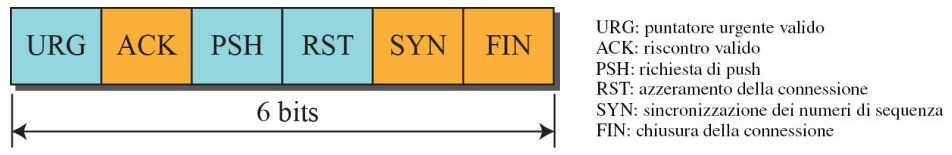
\includegraphics[width=13cm]{images/flag-di-controllo.JPG}
        \caption{Flag di controllo}
        \label{fig:flag-controllo}
    \end{figure}
    
    \item \textit{Dimensione della finestra.} Campo a 16 bit che indica la dimensione della finestra di cui l'altro host coinvolto nella trasmissione deve disporre.
    \item \textit{Checksum.} Campo a 16 bit contenente il checksum.
    \item \textit{Puntatore urgente.} Campo a 16 bit operativo se il flag URG (urgente) è attivato. Il campo contiene il numero che deve essere sommato al numero di sequenza per ottenere il numero dell'ultimo byte urgente nella sezione dati del segmento.
    \item \textit{Opzioni.} Vi possono essere da 0 a 40 byte di informazioni opzionali nell'intestazione del pacchetto TCP.
\end{itemize}

\subsection{Connessione TCP}
Il protocollo TCP è orientato alla connessione, ovvero stabilisce un percorso virtuale fra il mittente e il destinatario. Tutti i segmenti appartenenti a un messaggio vengono spediti lungo questo percorso logico. Utilizzare un percorso virtuale per l'intero messaggio semplifica il processo di conferma e di ritrasmissione dei segmenti smarriti o danneggiati. Ci si potrebbe chiedere come TCP possa essere orientato alla connessione dato che utilizza i servizi di IP, un protocollo privo di connessioni. In realtà la connessione TCP è virtuale, non fisica: TCP opera a un livello più alto, utilizza i servizi di IP per consegnare i singoli segmenti al destinatario, ma è il TCP stesso che controlla la connessione. Un segmento smarrito o danneggiato viene ritrasmesso da TCP, ma IP è inconsapevole di tale ritrasmissione. Un segmento ricevuto fuori sequenza viene bufferizzato da TCP fino a quando riceve il segmento mancante: IP è ignaro di questo riordinamento.

La trasmissione orientata alla connessione nel protocollo TCP richiede tre fasi: apertura della connessione, trasmissione dei dati e chiusura della connessione.

\subsubsection{Apertura della connessione}
TCP trasmette i dati in modalità tull-duplex: due entità TCP connesse in due macchine differenti sono in grado di trasmettere dati l'una all'altra simultaneamente. Questo comporta che ciascuna entità deve inizializzare la comunicazione e ottenere l'approvazione dell'entità corrispondente prima di poter trasferire qualsiasi dato.

La procedura di apertura della connessione in TCP è detta three way handshake (stretta di mano a tre vie). Consideriamo un esempio in cui un programma applicativo, chiamato client, vuole collegarsi a un altro programma applicativo, chiamato server, usando il protocollo di livello trasporto TCP. Il processo server deve essere attivo, e pronto ad accettare connessioni mediante il livello TCP, per cui deve richiedere al TCP una apertura passiva. Nonostante il server TCP sia in grado di aprire connessioni con un qualsiasi dispositivo connesso alla rete mondiale, non può aprire la connessione da solo, ma dietro richiesta di un processo applicativo. La richiesta fatta dal processo client, invece, è detta richiesta di apertura attiva: un processo client che voglia aprire una connessione con un processo server su un particolare dispositivo ne informa il suo TCP, il quale dà inizio alla procedura three way handshake.

Per illustrare la procedura si utilizzano due linee temporali, una per ciascuna postazione. Ogni segmento ha i valori appropriati per tutti i campi dell'intestazione (ed eventualmente anche per alcuni dei suoi campi opzionali): il numero di sequenza, il numero di riscontro, i flag di controllo (solo quelli utilizzati) e la dimensione della finestra (quando significativa). La procedura comporta i tre passi seguenti.
\begin{enumerate}
    \item Il client invia il primo segmento, un segmento SYN nel quale viene impostato il solo flag SYN, che serve per la sincronizzazione dei numeri di sequenza. Il client sceglie un numero random come primo numero di sequenza, chiamato numero di sequenza iniziale, o ISN (Initial Sequence Number), e lo invia al server. Si noti che questo segmento non contiene alcun numero di riscontro e non definisce la dimensione della finestra: quest'ultima è significativa solo nel caso in cui il segmento include un riscontro. Si noti che il segmento SYN è un segmento di controllo e non contiene dati utente, tuttavia usa un numero di sequenza: quando inizierà il trasferimento dei dati, il numero di sequenza verrà incrementato di un'unità. Si potrebbe dire che il segmento SYN non trasporta dati reali, ma solo un byte immaginario.

    \item Il server invia il secondo segmento, un segmento con i due flag SYN e ACK attivati. Il suo scopo è duplice: in primo luogo è un segmento SYN per la comunicazione nell'altra direzione. Il server utilizza questo segmento per inizializzare il numero di sequenza necessario per numerare i byte inviati dal server al client. In secondo luogo il server usa il segmento per riscontrare la ricezione del segmento SYN dal client impostando il flag ACK e indicando il prossimo numero di sequenza che si aspetta di ricevere dal client. Dato che contiene un riscontro, deve anche definire la dimensione della finestra di ricezione (\verb|rwnd|) che il client dovrà utilizzare. Essendo un segmento SYN esso deve essere confermato, quindi usa un numero di sequenza.

    \item Il client invia il terzo segmento, un segmento ACK, che conferma l'avvenuta ricezione del secondo segmento mediante il flag ACK. Si noti che il segmento ACK non usa alcun numero di sequenza se non contiene dati utenti, ma alcune implementazioni consentono a questo terzo segmento, nella fase di apertura della connessione, di trasportare i primi dati dal client: in questo caso si deve utilizzare un numero di sequenza per indicare il numero del primo byte nei dati.
\end{enumerate}

\begin{figure}[ht]
    \centering
    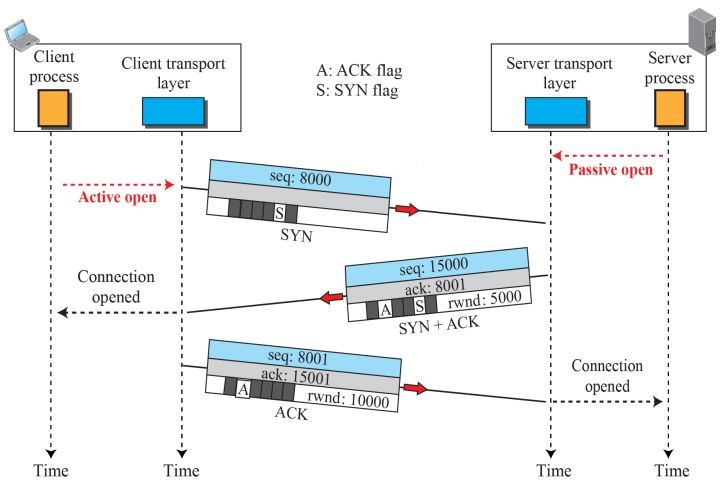
\includegraphics[width=11cm]{images/apertura-connessione-tcp.JPG}
    \caption{Apertura della connessione mediante il tree-way handshake}
    \label{fig:apertura-connessione-tcp}
\end{figure}

\subsubsection{Trasferimento dei dati}
Dopo aver stabilito la connessione è possibile trasferire i dati. Il client e il server possono inviare dati e riscontri in entrambe le direzioni. I dati che viaggiano nella medesima direzione dei riscontri sono trasportati nel medesimo segmento (in piggybacking). Viene illustrato un esempio, in cui il client, dopo aver aperto la connessione, invia 2000 byte di dati in due segmenti. Il server invia successivamente 2000 byte in un segmento; il client invia infine un nuovo segmento. I primi tre segmenti trasportano sia dati che riscontri, mentre l'ultimo segmento trasporta solo un riscontro perché non vi sono altri dati da trasmettere. Si notino i valori dei numeri di sequenza e di riscontro. I segmenti dati inviati dal client hanno il flag PSH (push - spingi) impostato, così che il server TCP sa di dover consegnare i dati al processo server non appena li riceve. Il segmento dal server, invece, non ha il flag PSH impostato.

\begin{itemize}
    \item \textit{Pushing dei dati.} Come si è già visto, il protocollo TCP mittente memorizza in un buffer i dati provenienti dal programma applicativo; la quantità di dati del buffer che vengono inseriti in un segmento è scelta a discrezione del protocollo TCP. Anche il protocollo TCP ricevente memorizza i dati ricevuti in un buffer e li trasmette al programma applicativo quando questo è pronto alla ricezione oppure quando il TCP lo ritiene conveniente. Questo modo d'operare così flessibile permette di migliorare l'efficienza delle procedure di trasmissione.

    Vi sono casi, però, in cui il programma applicativo non può operare in regime di flessibilità: si supponga che un processo interagisca direttamente con un altro processo all'altro capo della connessione. Il primo può voler inviare un comando al secondo e aspettarsi una risposta immediata; ritardi nella trasmissione o nella consegna della risposta possono non essere tollerati da questo programma.

    Il TCP gestisce queste operazioni con la funzione push che può essere richiesta dal mittente. In questo caso il TCP mittente non deve attendere che la finestra sia piena: deve, invece, creare e inviare immediatamente il segmento. Il TCP mittente, inoltre, deve attivare il bit PSH per segnalare al TCP ricevente che i dati contenuti nel segmento devono essere consegnati al più presto possibile al processo destinatario.

    \item \textit{Dati urgenti.} TCP è un protocollo orientato al flusso. I dati provenienti dal processo giungono al protocollo TCP come un flusso di caratteri e ogni byte di dati occupa una determinata posizione all'interno del flusso. Vi sono casi, però, in cui un processo ha la necessità di inviare dati urgenti; in altri termini il processo desidera che una porzione dei dati venga elaborata dal TCP prima degli altri indipendentemente dalla sua posizione nel flusso. La soluzione consiste nell'invio di un segmento con il bit URG attivato: il processo mittente notifica al TCP mittente che i dati sono urgenti; questi crea un segmento e inserisce i dati urgenti all'inizio del campo dati. Il resto del segmento può contenere datı normali dal buffer. Il campo puntatore urgente nell'intestazione indica la fine dei dati urgenti e l'inizio di quelli normali. Per esempio se il numero di sequenza del segmento vale 15000 e il valore del campo puntatore urgente è 200, il primo byte dei dati urgenti è il byte 15000 e l'ultimo byte è il 15200. I byte restanti nel segmento, se ve ne sono, sono dati non urgenti.
\end{itemize}

\begin{figure}[ht]
    \centering
    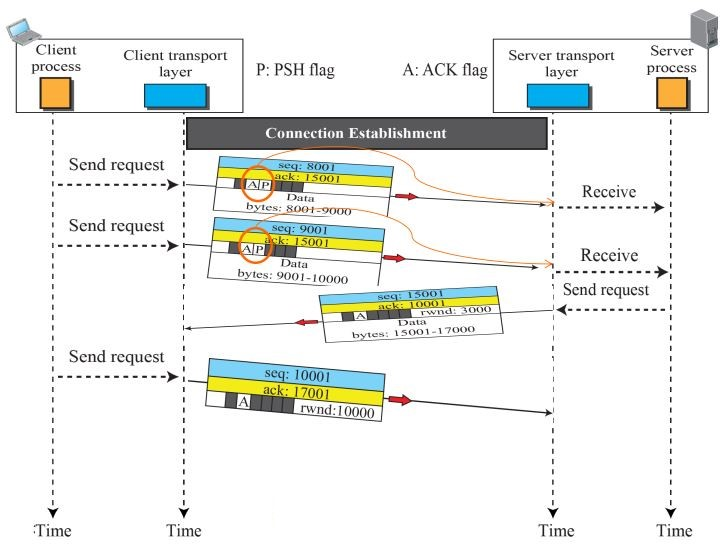
\includegraphics[width=11cm]{images/trasferimento-dati-tcp.JPG}
    \caption{Tasferimento dati}
    \label{fig:trasferimento-dati-tcp}
\end{figure}

\subsubsection{Chiusura della connessione}
Ciascuna delle due parti coinvolta nello scambio dei dati (client o server) può chiudere la connessione, sebbene la chiusura sia solitamente iniziata dal client. La maggior parte delle implementazioni attuali fornisce due opzioni per la chiusura della connessione: handshake a tre vie e handshake a quattro vie con l'opzione di half-close. Con handshake a tre vie:
\begin{enumerate}
    \item In questo caso, il client TCP, dopo aver ricevuto un comando di chiusura dal processo applicativo client, invia un primo segmento FIN nel quale viene impostato il flag FIN. Si noti che il segmento FIN può contenere l'ultima parte dei dati inviati dal client o può essere un semplice segmento di controllo. Se si tratta di un segmento di controllo, usa un solo numero di sequenza perché richiede un riscontro.
    \item Il server TCP, dopo aver ricevuto il segmento FIN, notifica la situazione al suo processo applicativo e invia il segmento FIN + ACK, per riscontrare la ricezione del segmento FIN al client e per annunciare la chiusura della connessione nella direzione opposta. Questo segmento può anche contenere gli ultimi dati da parte del server, se non trasporta dati, consuma solo un numero di sequenza perché è necessario riscontrarne la ricezione.
    \item Il client TCP invia l'ultimo segmento dell'handshake, un segmento ACK, per riscontrare la ricezione del segmento FIN dal server TCP. Questo segmento contiene il numero di riscontro, che vale uno più il numero di sequenza ricevuto nel segmento FIN dal server, non può trasportare dati e non consuma numeri di sequenza.
\end{enumerate}

\begin{figure}[ht]
    \centering
    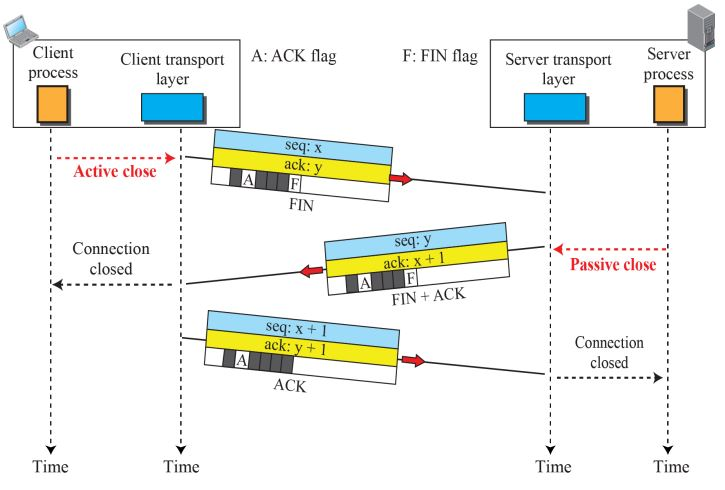
\includegraphics[width=11cm]{images/chiusura-connessione-tcp.JPG}
    \caption{Chiusura della connessione mediante three-way handshake}
    \label{fig:chiusura-connessione-tcp}
\end{figure}

Con half-close (chiusura a metà), in TCP, uno dei due processi può smettere di inviare dati mentre ne sta ancora ricevendo. Sebbene entrambe le entità possano eseguire la half-close, essa è solitamente iniziata dal client. Questo può avvenire quando il server ha bisogno di tutti i dati prima di poter procedere alla loro elaborazione. Il client richiede la half-close della connessione inviando un segmento FIN. Il server accetta la richiesta di chiusura inviando un segmento ACK. Il trasferimento dei dati dal client al server termina, ma il server può continuare a inviare dati. Quando il server ha terminato l'invio dei dati elaborati, invia un segmento FIN, che viene riscontrato da un segmento ACK dal client. Dopo il completamento della half-close è ancora possibile trasmettere i dati dal server al client e i riscontri dal client al server, ma il client non può inviare altri dati.

\begin{figure}[ht]
    \centering
    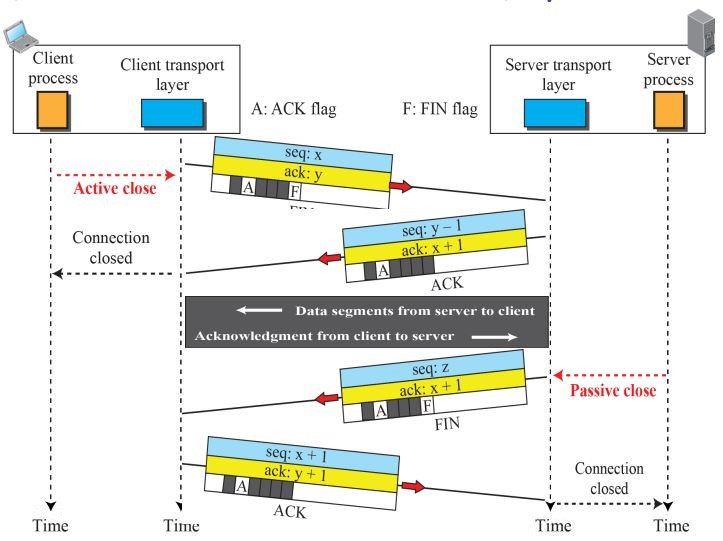
\includegraphics[width=11cm]{images/half-close.JPG}
    \caption{Half-close}
    \label{fig:half-closes}
\end{figure}

\subsection{Controllo degli errori}
Presentiamo ora un esempio che illustra bene i numeri di sequenza e di acknowledgment di TCP.
\begin{Example}{Numeri di sequenza e di acknowledgment di TCP}{}
    \textit{Supponiamo che l'Host A inizi una sessione Telnet con l'Host B. Il primo viene etichettato come client, il secondo come server. Ogni carattere immesso dall'utente (nel client) verrà spedito all'host remoto; quest'ultimo restituirà una copia di ciascun carattere, che sarà mostrata sullo schermo dell'utente. Questo “eco” viene utilizzato per assicurarsi che i caratteri visibili all'utente siano già stati ricevuti ed elaborati nel sito remoto. Quindi, nel lasso di tempo che intercorre tra la digitazione sul tasto e la visualizzazione sul monitor, ciascun carattere attraversa la rete due volte.}
    
    \begin{minipage}{\textwidth}
        \centering
        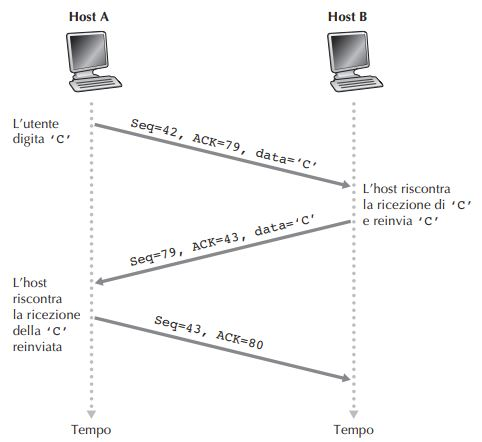
\includegraphics[width=0.6\textwidth]{images/es-controllo-errori.JPG}
        %\captionof{figure}{Esempio}
    \end{minipage}
    
    Supponiamo ora che l'utente digiti la lettera 'C' ... e poi vada a bere un caffè. Esaminiamo i segmenti TCP scambiati tra client e server. Ipotizziamo che i numeri di sequenza iniziali siano rispettivamente 42 e 79 per client e server. Ricordiamo che il numero di sequenza di un segmento è il numero di sequenza del primo byte nel campo dati. Pertanto, il primo segmento inviato dal client avrà numero di sequenza 42 e quello inviato dal server 79. Ricordiamo che il numero di acknowledgment è il numero di sequenza del successivo byte di dati che l'host sta aspettando. Dopo l'instaurazione della connessione TCP, ma prima dell'invio dei dati, il client è in attesa del byte 79 e il server del byte 42. Vengono spediti tre segmenti. Il primo è inviato dal client al server e contiene nel campo dati il byte ASCII per la lettera 'C'. Il campo numero di sequenza del primo segmento contiene 42. Inoltre, visto che il client non ha ancora ricevuto dati dal server, questo primo segmento avrà 79 nel proprio campo numero di acknowledgment. Il secondo segmento spedito dal server al client ha un duplice scopo. Innanzitutto, fa un acknowledgment dei dati ricevuti dal server. Ponendo 43 nel campo acknowledgment, il server indica al client di aver ricevuto con successo i primi 42 byte e di attendere i byte da 43 in poi. L'altra finalità di questo segmento è di mandare indietro un “eco” della lettera 'C'. Di conseguenza, il secondo segmento presenta nel proprio campo dati la lettera 'C', in ASCII, e ha numero di sequenza 79, ossia il numero iniziale del flusso di dati da server al client in questa connessione TCP, dato che si tratta proprio del primo byte di dati spedito dal server. Notiamo che il riscontro dei dati dal client al server viene trasportato in un segmento che a sua volta trasporta dati dal server al client; in gergo, si dice che tale acknowledgment è piggybacked (o anche in piggyback) sul segmento dati dal server al client. Il terzo segmento viene inviato dal client al server e ha come unico scopo dare un acknowledgment ai dati inviati dal server. Ricordiamo che il secondo segmento conteneva dati, la lettera 'C' dal server al client. Al contrario, il campo dati di questo segmento è vuoto (in altre parole, l'acknowledgment non è in piggyback ad alcun dato da client al server). Il segmento ha 80 nel suo campo numero di acknowledgment, in quanto il client ha ricevuto il flusso di byte fino al numero di sequenza 79 e ora è in attesa dei byte dall'80 in avanti. Si potrebbe considerare strano che questo segmento abbia un numero di sequenza pur senza contenere dati. In ogni caso, dato che TCP prevede un campo numero di sequenza, il segmento deve averne uno.
\end{Example}

Il protocollo TCP è un protocollo di trasporto affidabile; ovvero garantisce al livello applicazione che i dati inviati verranno consegnati nel giusto ordine, senza errori, senza smarrimenti o duplicazioni.

Il controllo degli errori garantisce affidabilità e prevede meccanismi per l'individuazione e la rispedizione dei segmenti corrotti, per la rispedizione dei segmenti smarriti, per l'identificazione e lo scarto dei segmenti duplicati e per la memorizzazione dei segmenti ricevuti fuori sequenza fino a quando non arrivano i segmenti mancanti. I tre semplici strumenti usati dal protocollo TCP per individuare gli errori di trasmissione sono il checksum, i messaggi di riscontro e il timeout.

\subsubsection{Checksum}
Il protocollo TCP prevede che ciascun segmento contenga un campo checksum di 16 bit, utilizzato per identificare i segmenti corrotti. Se un segmento è corrotto, questo viene ignorato dal destinatario e considerato smarrito. TCP utilizza un checksum di 16 bit, obbligatorio in ogni segmento.

\subsubsection{Riscontri}
TCP utilizza i riscontri per confermare la ricezione dei segmenti dati e dei segmenti di controllo che non contengono dati ma che usano un numero di sequenza. I segmenti di riscontro (ACK) non sono mai riscontrati.

Quando, il destinatario, genera i riscontri? Nell'evoluzione di TCP sono state definite varie regole, utilizzate poi da varie implementazioni. Di seguito si riportano le regole più comuni:
\begin{enumerate}
    \item Quando un'entità invia un segmento dati all'entità corrispondente, deve includere (piggybacking) un riscontro che fornisca il prossimo numero di byte che prevede di ricevere. Questa regola diminuisce il numero di segmenti necessari e riduce quindi il traffico.
    \item Quando il destinatario non ha dati da inviare e riceve un segmento nell'ordine corretto (ovvero con il numero di sequenza atteso) e il segmento precedente è già stato riscontrato, ritarda l'invio del segmento ACK fino a quando non arriva un altro segmento o fino a quando non scade un tempo massimo predefinito (normalmente di 500ms). In altre parole il destinatario ritarda l'invio di un segmento ACK se ha un unico segmento nella sequenza corretta da riscontrare. Anche questa regola (detta ACK posticipato o delayed) evita che i segmenti ACK creino un traffico eccessivo, e fa uso di un timer di ACK-posticipato.
    \item Quando arriva un segmento con numero di sequenza atteso e il segmento precedente non è stato riscontrato, il destinatario invia immediatamente un segmento ACK. In altre parole, non ci devono mai essere più di due segmenti nell'ordine corretto non riscontrati. Questo serve a evitare l'inutile ritrasmissione dei segmenti, che potrebbe produrre congestione nella rete.
    \item Quando arriva un segmento fuori sequenza, il destinatario invia immediatamente un segmento ACK notificando il numero di sequenza atteso nel prossimo segmento. Questo consente la ritrasmissione rapida (fast retransmission) di eventuali segmenti smarriti.
    \item Quando arriva un segmento mancante, il destinatario invia un segmento ACK per notificare il prossimo numero di sequenza atteso. Questo serve a notificare al mittente l'avvenuta ricezione di un segmento precedentemente annunciato come smarrito.
    \item Quando arriva un segmento duplicato, il destinatario lo scarta e invia immediatamente un riscontro con il numero di sequenza del prossimo segmento atteso. Questo risolve alcuni problemi legati alla perdita dei segmenti di conferma.
\end{enumerate}

\subsubsection{Ritrasmissione dei segmenti}
Il cuore del meccanismo di controllo degli errori è la ritrasmissione dei segmenti: quando un segmento viene inviato, viene memorizzato in una coda in attesa di essere riscontrato. Alla scadenza del timer di ritrasmissione o quando il mittente riceve tre ACK duplicati per il precedente segmento nella coda, quel segmento viene ritrasmesso. Analizziamo ora i due casi nel dettaglio.

Il TCP mittente inizializza un timer di ritrasmissione, o RTO (Retransmission Time-Out), per ogni segmento inviato. Allo scadere del tempo limite senza averne ricevuto un riscontro, il segmento all'inizio della coda (il segmento con il numero di sequenza inferiore) viene ritrasmesso e si la ripartire il timer. Si noti che si ipotizza sempre che $S_f < S_n$. RTT è il tempo necessario a un segmento per raggiungere il destinatario sommato al tempo necessario al relativo riscontro per raggiungere il mittente.

La regola relativa alla ritrasmissione dei segmenti è sufficiente se il valore di RTO non è eccessivo. A volte, tuttavia, viene smarrito un segmento e il destinatario riceve un numero tanto elevato di segmenti fuori sequenza da non poterli memorizzare (per la dimensione limitata del buffer). Per risolvere questo problema, la maggior parte delle implementazioni attuali osservano la regola dei tre ACK duplicati e ritrasmettono immediatamente il segmento mancante. Questa funzione viene chiamata ritrasmissione veloce. Con questa versione quando vengono ricevuti tre ACK duplicati (ovvero l'ACK originale più tre copie identiche) di un segmento, quello successivo viene immediatamente ritrasmesso senza attendere il timeout. Quando un segmento viene ritardato, smarrito o scartato, i segmenti che lo seguono giungono fuori sequenza (non nell'ordine atteso). La maggior parte delle implementazioni attuali del TCP non scartano i segmenti fuori sequenza, ma li memorizzano temporaneamente in attesa di ricevere il segmento mancante. Si noti tuttavia che i segmenti fuori sequenza non possono essere trasmessi al processo, dato che TCP garantisce la consegna dei dati nell'ordine corretto.

I dati possono arrivare fuori sequenza ed essere temporaneamente memorizzati dall'entità TCP destinataria, ma TCP garantisce al processo applicativo la consegna dei dati nell'ordine corretto.

\subsubsection{FSM per il trasferimento dei dati in TCP}
Il trasferimento dei dati in TCP riprende il Selective Repeat con alcune analogie con il GBN.

Nelle FSM si ipotizza che la comunicazione sia unidirezionale, ignorando qualsiasi aspetto relativo alla comunicazione bidirezionale. Si ipotizza inoltre che i segmenti siano riscontrati con segmenti ACK, ignorando i riscontri selettivi e il controllo della congestione. 

Dal lato del mittente, esistono alcune differenze con quella discussa per il protocollo SR. Una differenza è relativa alla ritrasmissione veloce (i tre ACK duplicati), l'altra all'aggiustamento della dimensione della finestra sulla base del valore di \verb|rwnd| (ignorando per il momento il problema del controllo della congestione). Dal lato del destinatario, le differenze fra la FSM con quella discussa per il meccanismo SR sono relative al ritardo dei riscontri nella comunicazione unidirezionale, e all'invio dei riscontri duplicati per consentire al mittente di effettuare la ritrasmissione veloce.

\begin{figure}[ht]
    \centering
    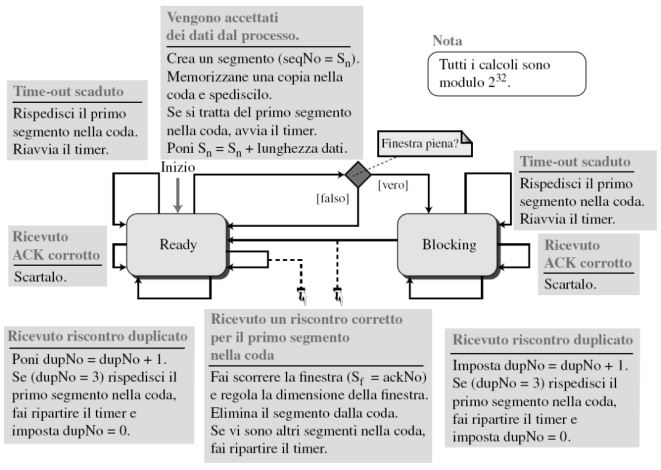
\includegraphics[width=0.50\textwidth]{images/mitt-controllo-errori.JPG}
    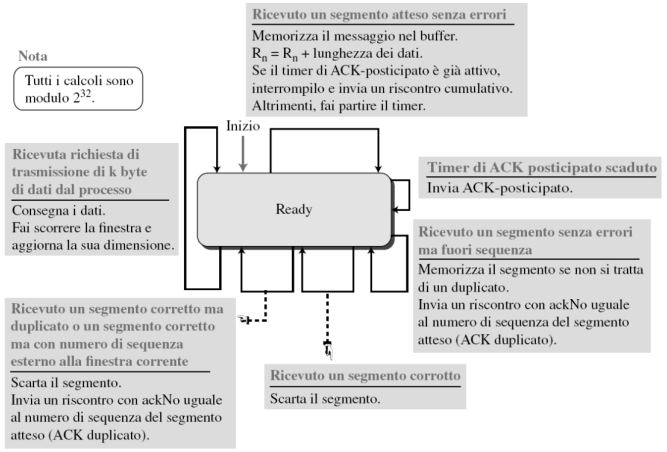
\includegraphics[width=0.49\textwidth]{images/dest-controllo-errori.JPG}
    \caption{FSM semplificata per il mittente e destinatario TCP}
    \label{fig:mitt-dest-controllo-errori}
\end{figure}

E' necessario enfatizzare anche che la FSM bidirezionale per il destinatario non è semplice come quella per il meccanismo SR, è necessario considerare alcune strategie come l'invio di un riscontro immediato quando il destinatario ha dei dati da trasmettere.

\subsubsection{Alcuni scenari}
In questo paragrafo si discutono alcuni esempi di situazioni che possono avvenire nelle operazioni del protocollo TCP, considerando esclusivamente gli aspetti relativi al controllo degli errori. In questi esempi i segmenti sono indicati con rettangoli. Se il segmento trasporta dati, vengono indicati l'intervallo dei numeri dei byte contenuti e il valore del campo riscontro. Se trasporta solo il riscontro, si indica solamente il numero di riscontro in un rettangolo più piccolo.

\begin{Example}{Operatività normale}{}
    \textit{Il primo scenario illustra il trasferimento di dati bidirezionali fra due sistemi. Il client TCP invia un segmento, il server TCP ne invia tre.}
    
    \begin{minipage}{\textwidth}
        \centering
        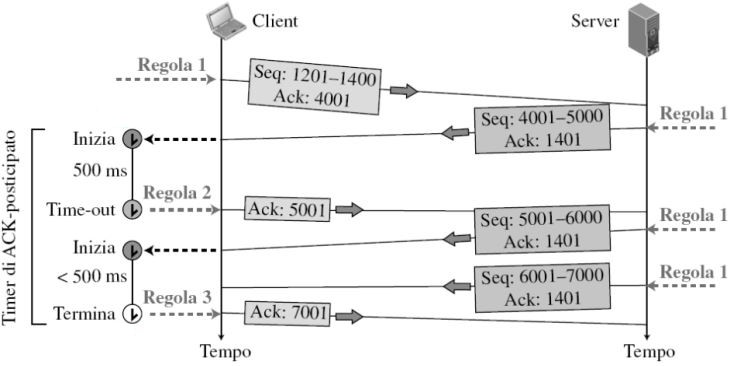
\includegraphics[width=0.7\textwidth]{images/normale-operativita.JPG}
        %\captionof{figure}{Esempio}
    \end{minipage}
    
    Per il primo segmento del client e tutti e tre i segmenti del server si applica la prima regola: vi sono dati da inviare, quindi il segmento indica il prossimo byte atteso. Quando il client riceve il primo segmento dal server, non ha altri dati da inviare: invia dunque un segmento ACK. Tuttavia la seconda regola stabilisce che il riscontro sia ritardato (posticipato) di 500ms in attesa di eventuali altri segmenti. Alla scadenza del timer viene inviata la conferma, dato che il client non può sapere se stanno arrivando altri segmenti e non può ritardare indefinitamente il riscontro. All'arrivo del segmento successivo viene inizializzato un altro timer di ACK posticipato. Questa volta, prima che scada il tempo impostato, arriva il terzo segmento che comporta l'invio del riscontro in conformità alla terza regola. Il timer RTO non è stato considerato, poiché nessun segmento è stato smarrito o ritardato. Si assume semplicemente che il timer RTO sia gestito correttamente.
\end{Example}

\begin{Example}{Segmento smarrito}{}
    \textit{In questo scenario si illustra il caso in cui un segmento viene smarrito o corrotto.} 
    
    I casi di segmento smarrito o corrotto vengono trattati nello stesso modo dal destinatario: il segmento smarrito viene perso da qualche parte nella rete, il segmento corrotto viene eliminato dal destinatario stesso. Entrambi vengono considerati persi. La figura illustra il caso in cui il segmento viene smarrito o eliminato da qualche router nella rete, eventualmente a causa di congestione. 

    \begin{minipage}{\textwidth}
        \centering
        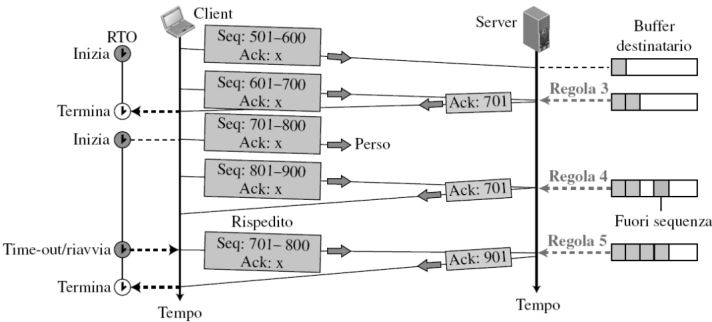
\includegraphics[width=0.7\textwidth]{images/segmento-smarrito.JPG}
        %\captionof{figure}{Esempio}
    \end{minipage}
    
    Si suppone che il trasferimento dei dati sia unidirezionale: una postazione trasmette, l'altra riceve. In questo scenario il mittente invia i segmenti 1 e 2 che sono immediatamente riscontrati con un ACK (regola 3). Il terzo segmento viene smarrito. Il destinatario riceve il segmento 4 che risulta fuori sequenza, ne memorizza i dati nel suo buffer ma lascia uno spazio per indicare che non vi è continuità nei dati. Invia immediatamente un riscontro al mittente indicando il prossimo byte atteso (regola 4). Si noti che l'entità TCP destinataria memorizza i byte da 801 a 900, ma non li consegna all'applicazione fino a quando non riceve i dati mancanti.

    L'entità TCP destinataria consegna al processo applicativo solo dati correttamente ordinati.

    Il TCP mittente mantiene un timer RTO per tutto il periodo di connessione. Alla scadenza del timer il TCP mittente ritrasmette il segmento 3, che questa volta arriva correttamente e viene riscontrato (regola 5).
\end{Example}

\begin{Example}{Ritrasmissione veloce}{}
    \textit{In questo scenario si vuole esemplificare il concetto di ritrasmissione veloce.} 
    
    Questo scenario è simile al precedente ad eccezione del valore di RTO che in questo caso è superiore.

    \begin{minipage}{\textwidth}
        \centering
        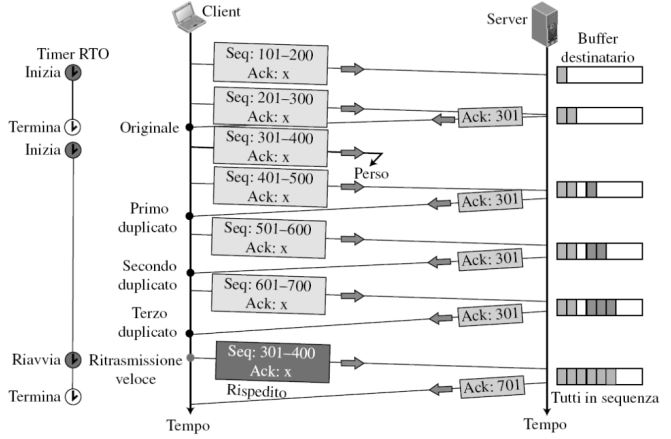
\includegraphics[width=0.7\textwidth]{images/ritrasmissione-rapida.JPG}
        %\captionof{figure}{Esempio}
    \end{minipage}

    Quando il destinatario riceve un qualsiasi segmento successivo a quello atteso (in questo caso il terzo segmento) invia un riscontro indicante il segmento atteso (regola 4). Il mittente riceve quattro riscontri con il medesimo valore (tre duplicati). Sebbene il timer non sia ancora scaduto, la regola di ritrasmissione veloce richiede che il segmento 3, il segmento indicato come atteso da tutti e quattro i riscontri, sia immediatamente ritrasmesso. Una volta ritrasmesso il segmento, il timer viene fatto ripartire.
\end{Example}

\begin{Example}{Riscontro smarrito senza ritrasmissione}{}
    \textit{Questo scenario illustra il caso in cui un riscontro smarrito viene automaticamente rimpiazzato dal successivo.}

    \begin{minipage}{\textwidth}
        \centering
        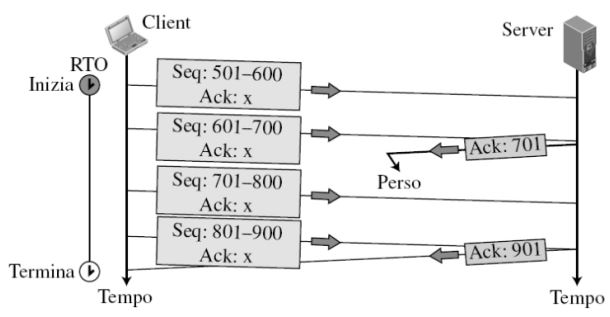
\includegraphics[width=0.5\textwidth]{images/riscontro-smarrito-senza-ritrasmissione.JPG}
        %\captionof{figure}{Esempio}
    \end{minipage}
    
    Con la tecnica di riscontro cumulativo utilizzata da TCP, la perdita di una conferma può passare inosservata al TCP mittente: il riscontro successivo corregge automaticamente lo smarrimento del riscontro.
\end{Example}

\begin{Example}{Riscontro smarrito con ritrasmissione}{}
    Se il riscontro successivo subisce un lungo ritardo o non vi è riscontro successivo (il riscontro smarrito è l'ultimo), il timer RTO scade senza che si sia ricevuto alcun riscontro. Il mittente ritrasmette quindi il segmento, che risulta duplicato. Il destinatario ignora il segmento che riceve duplicato ma ritrasmette immediatamente l'ultimo ACK per informare il mittente che il segmento o i segmenti sono arrivati a buon fine.

    \begin{minipage}{\textwidth}
        \centering
        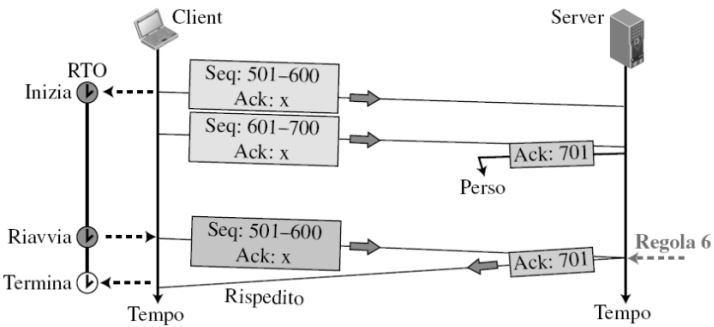
\includegraphics[width=0.5\textwidth]{images/riscontro-smarrito-con-ritrasmissione.JPG}
        %\captionof{figure}{Esempio}
    \end{minipage}

    Si noti che viene ritrasmesso solo un segmento sebbene due segmenti non siano stati riscontrati. Il mittente, alla ricezione dell'ACK ritrasmesso, capisce che entrambi i segmenti sono stati ricevuti correttamente dato che il riscontro è cumulativo.
\end{Example}


\subsection{Controllo del flusso}
Come già discusso, il controllo di flusso consente di bilanciare la velocità con cui un produttore genera i dati con la velocità con la quale un consumatore li utilizza. Il protocollo TCP separa il controllo di flusso dal controllo degli errori: si assume dunque che il canale logico fra il mittente e il destinatario TCP sia privo di errori.

\begin{figure}[ht]
    \centering
    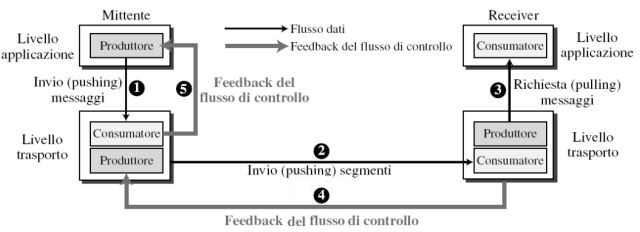
\includegraphics[width=11cm]{images/controllo-flusso-tcp.JPG}
    \caption{Flusso dei dati e feedback del controllo del flusso in TCP}
    \label{fig:controllo-flusso-tcp}
\end{figure}

La Figura \ref{fig:controllo-flusso-tcp} mostra che i dati generati dal processo applicativo mittente vengono prima passati (pushed) al TCP mittente, da questo trasmessi al TCP destinatario e infine da quest'ultimo al processo applicativo ricevente (percorsi 1, 2 e 3). I feedback del controllo di flusso, invece, vengono trasmessi dal TCP ricevente al TCP mittente e da questo al processo applicativo mittente (percorsi 4 e 5). La maggior parte delle implementazioni TCP non fornisce feedback del flusso di controllo dal processo destinatario al TCP destinatario, ma consente al processo destinatario di richiedere a suo piacimento i dati dal TCP destinatario. In altri termini il TCP destinatario controlla il TCP mittente, il quale a sua volta controlla il processo mittente.

Il feedback del controllo di flusso dal TCP mittente al processo applicativo mittente (percorso 5) è ottenuto tramite il semplice rifiuto dei dati da parte del TCP mittente quando la sua finestra è completa. La descrizione del controllo di flusso si concentra quindi sul feedback inviato dal TCP destinatario al TCP mittente (percorso 4).

\subsubsection{Apertura e chiusura delle finestre}
Per controllare il flusso, il TCP forza il mittente e il destinatario a regolare la dimensione delle proprie finestre, sebbene la dimensione del buffer di entrambe le parti venga fissata all'apertura della connessione. La finestra di ricezione si chiude (sposta la sua parete sinistra verso la destra) quando arrivano altri byte dal mittente, si apre (sposta la sua parete destra verso destra) quando vengono richiesti altri byte dal processo. Si ipotizza che non venga mai ridotta (ovvero che la parete destra non si sposti verso sinistra).

L'apertura, la chiusura e la riduzione della finestra di invio sono controllate dal destinatario. La finestra di invio si chiude (sposta la sua parete sinistra verso destra) quando ciò viene consentito da un nuovo riscontro, si apre (sposta la sua parete destra verso destra) quando la dimensione della finestra di ricezione (\verb|rwnd|) segnalata dal destinatario lo consente (nuovo ackNo + nuovo rvnd $>$ ultimo \verb|rwnd|). La finestra di invio viene ridotta quando non si verifica questa situazione.

\begin{figure}[ht]
    \centering
    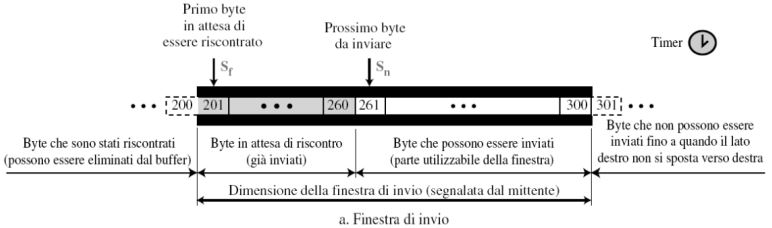
\includegraphics[width=12cm]{images/finestra-invio-tcp.JPG}
    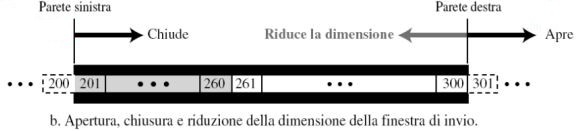
\includegraphics[width=10cm]{images/finestra-invio-tcp2.JPG}
    \caption{Finestra di invio nel protocollo TCP}
    \label{fig:finestra-invio-tcp}
\end{figure}

Si descrive ora come le finestre di invio e di ricezione vengano impostate nella fase di apertura della connessione e come vengano modificate nella fase di trasferimento dati. A tal proposito viene illustrato un semplice esempio.

\begin{Example}{Finestre di invio e recezione}{}
    \textit{Si illustra un semplice esempio di trasferimento dati unidirezionale (dal client al server). Per il momento si ignora il controllo degli errori, ipotizzando che nessun segmento venga corrotto, smarrito o arrivi duplicato o fuori sequenza.}
    
    \begin{minipage}{\textwidth}
        \centering
        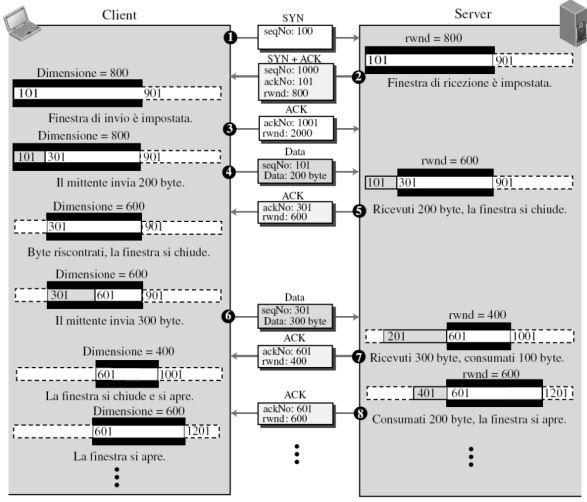
\includegraphics[width=0.6\textwidth]{images/es-finestra-invio.JPG}
        %\captionof{figure}{Esempio}
    \end{minipage}
    
    Si noti che si sono mostrate due sole finestre per il trasferimento dati unidirezionale. Sebbene il client definisca la dimensione della finestra del server di 2000 byte nel terzo segmento, tale finestra non è schematizzata nella figura poiché si tratta di comunicazione unidirezionale. Vengono trasmessi otto segmenti fra client e server.
    \begin{enumerate}
        \item Il primo segmento è dal client al server (un segmento \verb|SYN|) per richiedere l'apertura di una connessione. Il client annuncia il proprio numero di sequenza iniziale \verb|seqNo=100|. Quando il server riceve questo segmento, alloca un buffer di dimensione 800 (per ipotesi) e imposta la propria finestra per utilizzare l'intero buffer (\verb|rwnd=800|). Si noti che il numero del byte atteso successivo è il 101.
        \item Il secondo segmento, un \verb|SYN+ACK|, è dal server al client. Utilizza \verb|ackNo=101| per indicare che si attende di ricevere i byte a partire dal 101. Annuncia anche che il client può impostare una dimensione del buffer di 800 byte.
        \item Il terzo segmento è un \verb|ACK| dal client al server. Si noti che il client ha impostato la dimensione della finestra di ricezione con \verb|rwnd=2000|, ma nella figura questa finestra non viene indicata poiché si tratta esclusivamente il caso di comunicazione unidirezionale.
        \item Dopo che il client ha impostato la dimensione della propria finestra (800), come indicato dal server, il processo richiede la trasmissione di 200 byte di dati. Il client TCP numera questi byte da 101 a 300, crea un segmento e lo invia al server. Il segmento segnala che il numero del primo byte è 101 e che trasporta 200 byte di dati. La finestra del client viene quindi impostata in modo tale da indicare che sono stati inviati 200 byte di dati, che sono ancora da riscontrare. Il server quando riceve il segmento memorizza i dati e la finestra di ricezione si chiude per indicare che il byte successivo atteso è il numero 301; i byte memorizzati occupano 200 byte del buffer.
        \item  Il quinto segmento è il feedback dal server al client, con il quale il server riscontra i byte fino al 300 incluso (aspettandosi di ricevere il 301). Il segmento include anche la nuova dimensione della finestra di ricezione dopo il decremento (600). Il client, ricevuto questo segmento, elimina i byte confermati dalla propria finestra chiudendola, indicando che il byte successivo atteso è il 301. La dimensione della finestra, tuttavia, viene ridotta a 600 byte. Sebbene il buffer allocato possa contenere 800 byte, la finestra non si può aprire (spostare la parete destra verso destra) poiché il destinatario non lo consente.
        \item Il segmento 6 viene inviato dal client dopo che il suo processo chiede la trasmissione di altri 300 byte. Il segmento definisce \verb|seqNo=301| e contiene 300 byte. Il server, quando riceve questo segmento, ne memorizza i dati e deve ridurre la dimensione della propria finestra. Dopo che il proprio processo ha richiesto 100 byte di dati, la finestra chiude dalla sinistra per un ammontare di 300 byte, ma apre alla destra per un ammontare di 100 byte. Come risultato la sua dimensione viene ridotta di soli 200 byte, al valore attuale di 400 byte.
        \item Nel segmento 7 il server riscontra la ricezione dei dati e annuncia che la dimensione della propria finestra è 400. Quando il client riceve questo segmento, deve ridurre nuovamente la propria finestra e impostare la sua dimensione al valore \verb|rwnd=400| come indicato dal server. La finestra di invio si chiude a sinistra di 300 byte e si apre a destra di 100 byte.
        \item Anche il segmento 8 viene inviato dal server, dopo che il proprio processo ha richiesto altri 200 byte. Il server incrementa la dimensione della propria finestra (\verb|rwnd| vale ora 600) e informa il client che si attende ancora il byte 601, ma che la dimensione della propria finestra è ora di 600 byte. E' necessario precisare che la spedizione di questo segmento dipende dalle varie implementazioni. Alcune non consentono l'annuncio di \verb|rwnd| in questo momento: il server deve ricevere altri dati prima di poterlo fare. Il client, ricevuto questo segmento, apre la propria finestra di 200 byte senza chiuderla. Come risultato la dimensione della propria finestra diviene 600.
    \end{enumerate}
\end{Example}

Come già detto la finestra di ricezione non può essere ridotta. La finestra di invio, invece, può essere ridotta quando il destinatario definisce un valore di \verb|rwnd| inferiore al precedente. Alcune implementazioni non permettono comunque la riduzione della finestra di invio: questa limitazione non consente di spostare la parete destra della finestra di invio verso sinistra. In altri termini il destinatario deve rispettare la seguente relazione fra l'ultimo riscontro e il precedente e fra il precedente e il nuovo valore di \verb|rwnd| per evitare la riduzione della finestra di invio:
\begin{equation*}
    \verb|nuovo ackNo| + \verb|nuovo rwnd| \geq \verb|ultimo ackNo| + \verb|ultimo rwnd|
\end{equation*}

La parte sinistra della diseguaglianza rappresenta la nuova posizione della parete destra rispetto allo spazio dei numeri di sequenza; la parte destra indica la posizione precedente della parete destra. La relazione indica che la parete destra non deve spostarsi a sinistra. La diseguaglianza è necessaria al destinatario per controllare i propri annunci. Si noti tuttavia che la diseguaglianza è valida solo se $S_f<S_n$: si deve ricordare che tutti i calcoli vengono effettuati modulo $2^{32}$.

\subsection{Controllo della congestione}
TCP utilizza diverse strategie per gestire la congestione nella rete.

\subsubsection{Finestra di congestione}
Quando si è descritto il controllo di flusso nel protocollo TCP, si è detto che la dimensione della finestra di invio è controllata dal destinatario tramite il valore di \verb|rwnd|, che viene indicato in ogni segmento trasmesso nella direzione opposta. L'impiego di questa strategia garantisce che la finestra del ricevente non venga mai sovraccaricata con i dati ricevuti (non esiste congestione della postazione destinataria). Questo tuttavia non garantisce che i buffer intermedi, i buffer nei router, non si congestionino. Un router potrebbe ricevere dati da più di un mittente. Indipendentemente dalla capacità del buffer di un router, è sempre possibile che questo venga saturato e che si trovi costretto a scartare i segmenti di qualche specifico mittente TCP. In altre parole non vi è congestione agli estremi, ma vi può essere congestione nei nodi intermedi. TCP deve preoccuparsi della possibile congestione della rete poiché la perdita di un gran numero di segmenti può influire significativamente sul meccanismo di controllo degli errori. La perdita di numerosi segmenti comporta la loro rispedizione, peggiorando così la congestione della rete e portando alla fine al collasso della comunicazione.

TCP è un protocollo end-to-end che sfrutta i servizi di IP. La congestione nei router è un problema che riguarda IP e che dovrebbe essere gestito a livello rete. Tuttavia IP è un semplice protocollo senza controllo della congestione. TCP è dunque necessariamente costretto a occuparsi del problema.

TCP non può ignorare la congestione nella rete: non può inviare un numero di segmenti eccessivo alla rete, altrimenti ne verrebbe penalizzato. Ma TCP non può nemmeno essere troppo conservativo, nel senso di inviare un numero troppo limitato di segmenti nell'unità di tempo, poiché non sfrutterebbe al meglio la capacità della rete. TCP deve quindi prevedere delle strategie per accelerare la trasmissione dei dati quando non vi è congestione e ridurre la trasmissione quando rileva la congestione.

Per controllare il numero di segmenti da trasmettere, TCP utilizza una seconda variabile chiamata \verb|cwnd| (congestion window - finestra di congestione), il cui valore dipende dal livello di congestione nella rete. Le due variabili \verb|cwnd| e \verb|rwnd| congiuntamente definiscono la dimensione della finestra di invio di TCP. La prima variabile è legata alla congestione della rete, la seconda alla congestione delle postazioni terminali. La dimensione finale della finestra corrisponde al minimo dei due valori.

\begin{equation*}
    \text{\textit Dimensione della finestra} = min(rwnd, cwnd)    
\end{equation*}

\subsubsection{Rilevare la congestione}
Prima di analizzare come il valore di \verb|cwnd| debba essere impostato e aggiornato, è necessario descrivere come un mittente TCP possa identificare il possibile verificarsi della congestione nella rete. Il mittente interpreta come sintomi di congestione due eventi: il timeout e la ricezione di tre riscontri duplicati.

Il primo evento è dunque il timeout. Se un mittente TCP non riceve un riscontro per un segmento o un gruppo di segmenti prima dello scadere del timeout, suppone che tale segmento o i segmenti siano stati smarriti a causa della congestione.

Il secondo evento è la ricezione di tre riscontri duplicati (quattro ACK con il medesimo numero di riscontro). Si ricordi che un destinatario TCP invia un riscontro duplicato per segnalare un ritardo nella ricezione di un segmento, ma tre riscontri duplicati sono un'indicazione di segmento smarrito, che può essere dovuto a congestione nella rete. La congestione nel caso dei tre riscontri duplicati è tuttavia probabilmente meno critica che nel caso del timeout. Se il destinatario invia tre riscontri duplicati, significa che un segmento è stato smarrito, ma anche che altri tre segmenti sono stati ricevuti: la rete è al limite della congestione o è appena rientrata da una congestione.

E' interessante notare che il mittente TCP usa solo un tipo di feedback dal destinatario per rilevare la congestione: i riscontri. L'assenza della ricezione rapida e regolare dei riscontri, evidenziata dallo scadere del timeout, è il sintomo di una congestione severa; la ricezione di tre riscontri duplicati è il sintomo di una congestione debole.

\subsubsection{Strategie di gestione della congestione}
La strategia generale del protocollo TCP per gestire la congestione si basa su tre fasi: slow start (partenza lenta), congestion avoidance (prevenzione della congestione) e fast recovery (recupero veloce). Si descrive per prima ciascun algoritmo, per poi mostrare come il protocollo TCP passi dall'uno all'altro durante una connessione.

\begin{Algoritmo}{Slow start: incremento esponenziale}{}
    L'algoritmo slow start (partenza lenta) si basa sull'idea che la dimensione della finestra di congestione (\verb|cwnd|) viene inizializzata con la dimensione del segmento massimale (MSS - Maximum Segment Size), ma viene aumentata di un valore corrispondente a MSS a ogni segmento riscontrato. Come già visto, l'MSS viene determinato all'apertura della connessione utilizzando l'opzione omonima.

    Il nome dell'algoritmo è decisamente fuorviante: l'algoritmo parte lentamente ma procede con velocità esponenzialmente crescente. Si è supposto che \verb|rwnd| sia molto più elevato di \verb|cwnd|, in modo tale che la finestra del mittente sia sempre uguale a \verb|cwnd|. Si ipotizza anche che tutti i segmenti siano della stessa dimensione di MSS byte. Per semplicità si ignora anche la strategia dei riscontri in ritardo e si ipotizza che ogni segmento sia riscontrato individualmente.

    \begin{minipage}{\textwidth}
        \centering
        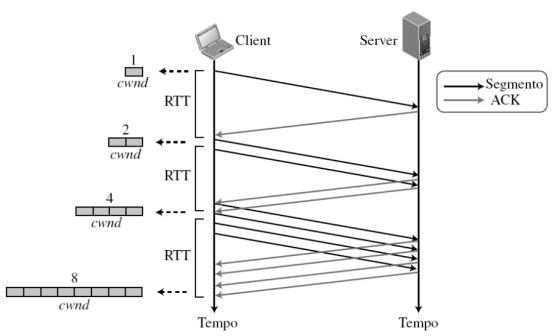
\includegraphics[width=0.7\textwidth]{images/slow-start.JPG}
        %\captionof{figure}{Esempio}
    \end{minipage}

    Il mittente inizia con \verb|cwnd=1|, quindi può inviare un solo segmento. Ricevuto il primo riscontro, il segmento riscontrato viene eliminato dalla finestra di invio: nella finestra si è quindi liberato spazio per un segmento. Anche la dimensione della finestra di congestione è incrementata di 1 perché la ricezione del riscontro è un buon sintomo di assenza di congestione nella rete. La dimensione della finestra vale ora 2 ed è possibile inviare due segmenti. Quando questi vengono confermati, la dimensione della finestra viene aumentata di 1 per ciascun riscontro ricevuto, quindi \verb|cwnd| vale ora 4 e così via. In altri termini, la dimensione della finestra di congestione con questo algoritmo è una funzione del numero di riscontri ricevuti e può essere determinata come segue:

    \begin{equation*}
        \textit{Se arriva un riscontro: } cwnd = cwnd+1        
    \end{equation*}

    Valutando la dimensione di \verb|cwnd| in funzione del tempo di andata e ritorno (RTT), si trova che la velocità di crescita è esponenziale, dunque molto aggressiva, in termini di ciascun RTT:

    \begin{align*}
        &Inizio&\rightarrow &\hspace{1.5cm}cwnd=1\rightarrow 2^0\\
        &Dopo 1 RTT&\rightarrow &\hspace{1.5cm}cwnd=cwnd+1=1+1=2\rightarrow 2^1\\
        &Dopo 2 RTT&\rightarrow &\hspace{1.5cm}cwnd=cwnd+2=2+2=4\rightarrow 2^2\\
        &Dopo 3 RTT&\rightarrow &\hspace{1.5cm}cwnd=cwnd+4=4+4=8\rightarrow 2^3
    \end{align*}

    La progressione dell'algoritmo non può continuare indefinitamente: è necessaria una soglia per arrestare questa fase. Il mittente tiene traccia di una variabile, chiamata \verb|ssthresh| (slow start threshold o soglia di slow start): quando la dimensione della finestra espressa in byte raggiunge questa soglia, slow start termina e inizia la fase successiva.
\end{Algoritmo}

E' necessario menzionare il fatto che la progressione dell'algoritmo slow start è più lenta nel caso di riscontri posticipati. Si ricordi che \verb|cwnd| è incrementato di 1 per ciascun riscontro. Di conseguenza, se due segmenti vengono riscontrati cumulativamente, il valore di \verb|cwnd| si incrementa solo di 1, non di 2. La crescita è ancora esponenziale, ma non è una potenza di 2.

La dimensione della finestra di congestione aumenta esponenzialmente nella fase di slow start, ma per evitare la congestione il ritmo di crescita deve essere rallentato. TCP prevede un altro algoritmo, chiamato congestion avoidance, che incrementa in modo lineare anziché esponenziale il valore di \verb|cwnd|.

\begin{Algoritmo}{Congestion avoidance: additive increase}{}
     Quando la dimensione della finestra di congestione raggiunge la soglia di slow start (\verb|ssthresh|) dove \verb|cwnd=i|, la fase di slow start si arresta e inizia la fase di incremento lineare (additive increase). Con questo algoritmo, ogni volta che viene riscontrata l'intera finestra di segmenti la dimensione della finestra di congestione viene incrementata di 1.

    \begin{minipage}{\textwidth}
        \centering
        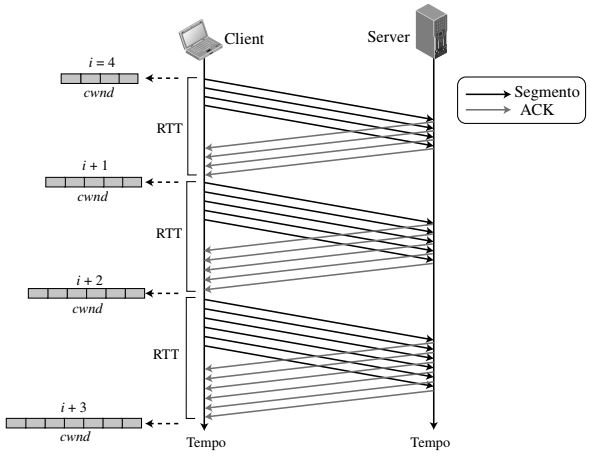
\includegraphics[width=0.7\textwidth]{images/congestion-avoidance.JPG}
        %\captionof{figure}{Esempio}
    \end{minipage}
    
    Il mittente inizia con \verb|cwnd=4|. Questo significa che il mittente può inviare solo quattro segmenti, prima di ricevere un riscontro. In questo caso, dopo che il mittente ha ricevuto i riscontri per tutti i segmenti della finestra, la dimensione della finestra viene aumentata di 1. La dimensione della finestra è quindi 5. Dopo aver inviato 5 segmenti e aver ricevuto i 5 riscontri corrispondenti, la dimensione della finestra di congestione diviene 6 e così via.

    Anche con questo algoritmo la dimensione della finestra di congestione è una funzione del numero di riscontri ricevuti e viene determinata come segue:

    \begin{equation*}
        \textit{Se arriva un riscontro: } cwnd = cwnd+(1/cwnd)
    \end{equation*}

    In altri termini, la dimensione della finestra cresce solamente di una porzione \verb|1/cwnd| di un MSS (in byte). Ovvero, tutti i segmenti nella finestra precedente devono essere riscontrati per aumentare la finestra di 1 MSS. Valutando la dimensione di \verb|cwnd| in termini del tempo di andata e ritorno (RTT), si trova che la velocità aumenta in modo lineare, ovvero molto più lentamente che nello slow start.

    \begin{align*}
        &Inizio&\rightarrow &\hspace{1.5cm}cwnd = i\\
        &Dopo 1 RTT&\rightarrow &\hspace{1.5cm}cwnd = i + 1\\
        &Dopo 2 RTT&\rightarrow &\hspace{1.5cm}cwnd = i + 2\\
        &Dopo 3 RTT&\rightarrow &\hspace{1.5cm}cwnd = i + 3\\
    \end{align*}

    Con l'algoritmo congestion avoidance, la dimensione della finestra di congestione viene aumentata linearmente fino alla rilevazione della congestione.
\end{Algoritmo}

\begin{Algoritmo}{Fast recovery}{}
    L'algoritmo fast recovery (recupero veloce) è opzionale in TCP. Esso inizia quando arrivano tre riscontri duplicati che vengono interpretati come indizio di leggera congestione nella rete. Come il congestion avoidance, anche questo algoritmo incrementa linearmente, ma incrementa la dimensione della finestra di congestione quando riceve un riscontro duplicato (dopo i tre riscontri duplicati che fanno partire questo algoritmo). Si può dire:

    \begin{equation*}
        \textit{Se arriva un riscontro duplicato: } cwnd = cwnd+(1/cwnd)
    \end{equation*}
\end{Algoritmo}

Sono state presentate tre tecniche di gestione della congestione in TCP. Si vuole ora capire quando viene utilizzata ciascuna di queste e quando TCP decide di passare dall'una all'altra. Per far questo è necessario fare riferimento a due versioni di TCP: Taho e Reno.

\subsubsection{TCP Taho}
La prima versione di TCP, chiamata TCP Taho, usava solo due algoritmi per la gestione della congestione: slow start e congestion avoidance.

\begin{figure}[ht]
    \centering
    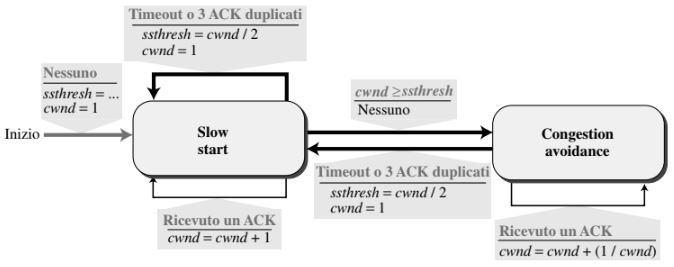
\includegraphics[width=10cm]{images/fsm-tcp-thao.JPG}
    \caption{FSM per il meccanismo di controllo della congestione di TCP Thao}
    \label{fig:tcp-thao}
\end{figure}

TCP Taho reagisce ai due sintomi di congestione, il timeout e i tre riscontri duplicati, nello stesso modo. In questa versione, una volta aperta la connessione, TCP avvia l'algoritmo slow start e imposta la variabile \verb|ssthresh| a un valore preconcordato (solitamente multiplo di MSS) e \verb|cwnd| a 1 MSS. In questo stato, come già detto, ogni volta che arriva un riscontro la dimensione della finestra di congestione viene aumentata di 1. E' evidente che si tratta di una strategia molto aggressiva che incrementa esponenzialmente la dimensione della finestra, cosa che può comportare una congestione. Se viene rilevata la congestione (scadenza del timeout o ricezione di tre riscontri duplicati), TCP interrompe immediatamente la crescita esponenziale, fa ripartire l'algoritmo slow start con nuovo threshold uguale alla metà del valore corrente di \verb|cwnd| e reimposta la dimensione della finestra a 1. In altri termini, non solo TCP riparte dall'inizio, ma aggiorna anche il threshold. Se non viene rilevata congestione fino al raggiungimento del threshold, TCP considera di avere raggiunto il massimo delle possibili ambizioni e di non potere continuare a ingrandire la finestra a tale velocità. Si sposta quindi nello stato di congestion avoidance, dove la dimensione della finestra viene incrementata di 1 ogni volta che riceve un numero di riscontri pari alla dimensione corrente della finestra. Per esempio, se la dimensione della finestra è di 5 MSS, è necessario ricevere altri 5 riscontri prima di poterla incrementare a 6 MSS. Si noti che non vi è un limite alla dimensione della finestra che può essere raggiunta in questo stato: la crescita lineare continua fino alla chiusura della connessione o fino a quando viene rilevata la congestione. Se la congestione viene rilevata in questo stato, TCP reimposta il valore di \verb|ssthresh| alla metà del valore corrente di \verb|cwnd| e si sposta nuovamente nello stato slow start.

Sebbene in questa versione di TCP la dimensione di \verb|ssthresh| venga continuamente aggiornata a ogni rilevazione di congestione, essa non diviene necessariamente minore del valore precedente. Per esempio, se il valore originale di \verb|ssthresh| fosse 8 MSS e la congestione fosse rilevata quando TCP è nello stato di congestion avoidance con valore di \verb|cwnd=20|, il nuovo valore di \verb|ssthresh| diverrebbe 10, ovvero verrebbe aumentato.

\begin{Example}{TCP Thao}{}
    \begin{minipage}{\textwidth}
        \centering
        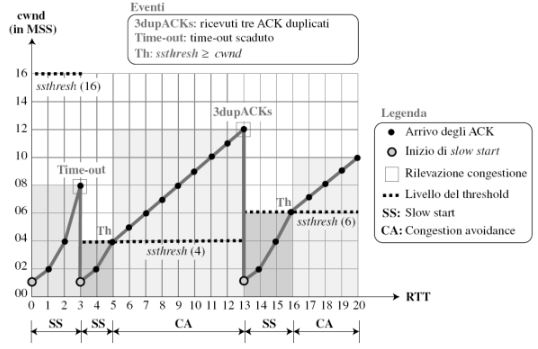
\includegraphics[width=0.6\textwidth]{images/es-tcp-thao.JPG}
        %\captionof{figure}{Esempio}
    \end{minipage}

    TCP inizia il trasferimento dei dati e imposta la variabile \verb|ssthresh| all'ambizioso valore di 16 MSS. Lo stato iniziale è lo slow start (SS) con \verb|cwnd=1|. La finestra di congestione cresce esponenzialmente ma avviene un timeout dopo il terzo RTT (prima di raggiungere il threshold). TCP assume che la rete sia congestionata, imposta il valore di \verb|ssthresh| a 4 MSS (la metà del valore corrente di \verb|cwnd|, che vale 8) e inizia un nuovo stato slow start (SS) con \verb|cwnd=1| MSS. La finestra di congestione cresce esponenzialmente fino a quando raggiunge il nuovo valore di threshold. A questo punto il TCP passa nello stato congestion avoidance (CA), dove la finestra di congestione cresce linearmente fino a quando raggiunge \verb|cwnd=12| MSS. A questo punto vengono ricevuti tre riscontri duplicati, un altro sintomo di congestione della rete. TCP dimezza nuovamente il valore di \verb|ssthresh| a 6 MSS e passa nello stato slow start (SS), La crescita esponenziale di \verb|cwnd| prosegue. Dopo RTT 15, la dimensione di \verb|cwnd| è 4 MS. Dopo avere inviato quattro segmenti e ricevuto due soli riscontri, la dimensione della finestra raggiunge il valore di \verb|ssthresh(6)|, quindi TCP passa nello stato congestion avoidance. Il trasferimento dei dati continua in questo stato (CA) fino a quando viene chiusa la connessione, in corrispondenza di RTT 20.    
\end{Example}

\subsubsection{TCP Reno}
In una versione più recente di TCP, chiamata Reno, è stato aggiunto un nuovo stato alla FSM per il controllo della congestione, chiamato stato di fast recovery (recupero veloce). Questa versione tratta i due sintomi della congestione, il timeout e la ricezione dei tre riscontri duplicati, in modo differente. Quando avviene un timeout, TCP passa allo stato slow start (o riparte in questo stato se già vi si trova). Quando riceve tre riscontri duplicati, TCP passa allo stato fast recovery e vi rimane fintantoché arrivano altri riscontri duplicati. Lo stato fast recovery è in un certo senso uno stato intermedio fra gli stati slow start e congestion avoidance. Si comporta come lo slow start, nel senso che \verb|cwnd| cresce esponenzialmente, ma il valore iniziale di \verb|cwnd| è uguale a \verb|ssthresh| più 3 MSS (anziché 1). Quando TCP passa nello stato fast recovery, possono avvenire tre eventi principali.
\begin{enumerate}
    \item Se continuano ad arrivare riscontri duplicati, TCP rimane nello stato ma \verb|cwnd| cresce esponenzialmente. 
    \item Se avviene un timeout, TCP assume che vi sia una reale congestione nella rete e passa allo stato slow start. 
    \item Se arriva un nuovo riscontro (non duplicato), TCP passa allo stato congestion avoidance, ma riduce il valore di \verb|cwnd| al valore di \verb|ssthresh| come se i tre riscontri duplicati non fossero stati ricevuti e la transizione fosse dallo stato slow start allo stato congestion avoidance.
\end{enumerate}

\begin{figure}[ht]
    \centering
    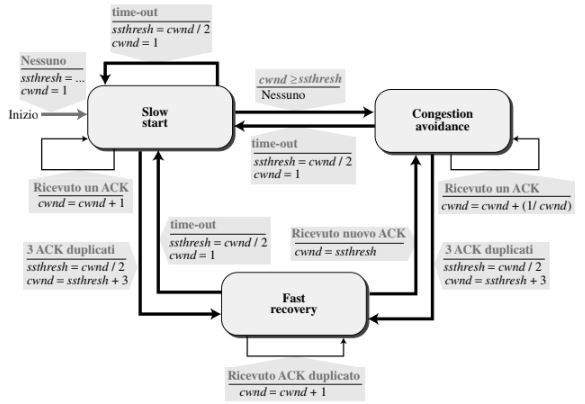
\includegraphics[width=10cm]{images/fsm-tcp-reno.JPG}
    \caption{FSM per il TCP Reno}
    \label{fig:tcp-reno}
\end{figure}

\begin{Example}{TCP Reno}{}
    \begin{minipage}{\textwidth}
        \centering
        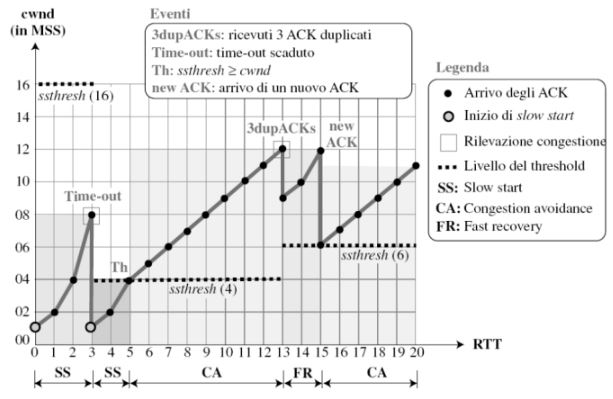
\includegraphics[width=0.6\textwidth]{images/es-tcp-reno.JPG}
        %\captionof{figure}{Esempio}
    \end{minipage}

    La dimensione della finestra di congestione cambia nello stesso modo fino a RTT 13, quando vengono ricevuti 3 riscontri duplicati. A questo punto TCP Reno riduce \verb|ssthresh| a 6 MSS (come nel caso del TCP Taho) ma imposta il valore di \verb|cwnd| a un valore molto più alto (\verb|ssthresh| + 3 = 9 MSS) anziché 1 MSS. TCP Reno passa ora nello stato di fast recovery. Si ipotizza che arrivino due altri ACK duplicati fino a RTT 15, mentre \verb|cwnd| cresce esponenzialmente. A questo punto arriva un nuovo riscontro (non duplicato) che segnala la ricezione del segmento smarrito. TCP Reno passa ora nello stato congestion avoidance, ma riduce prima la finestra di congestione a 6 MSS (il valore di \verb|ssthresh|), ignorando l'intero stato fast recovery e ritornando nella traccia precedente.    
\end{Example}

\subsection{Timeout e stima del tempo di andata e ritorno}
TCP utilizza un meccanismo di timeout e ritrasmissione per recuperare i segmenti persi. Sebbene tutto questo sia concettualmente semplice, l’implementazione di tale meccanismo in un protocollo come TCP crea alcuni problemi. Forse la questione più ovvia è la durata degli intervalli
di timeout. Chiaramente, il timeout dovrebbe essere più grande del tempo di andata e ritorno sulla connessione (RTT), ossia del tempo trascorso da quando si invia un segmento a quando se ne riceve l’acknowledgment, altrimenti ci sarebbero delle ritrasmissioni inutili. Ma di quanto deve essere maggiore? E, innanzitutto, come dovrebbe essere stimato RTT? Si dovrebbe associare un timer a ogni segmento non riscontrato?

\subsubsection{Stima del tempo di andata e ritorno}
Cominciamo lo studio della gestione dei timer TCP considerando come il protocollo stimi il tempo di andata e ritorno tra mittente e destinatario. L’RTT misurato di un segmento, denotato come SampleRTT, è la quantità di tempo che intercorre tra l’istante di invio del segmento (ossia quando viene passato a IP) e quello di ricezione dell’acknowledgment del segmento. Anziché misurare un SampleRTT per ogni segmento, la maggior parte delle implementazioni TCP effettua una sola misurazione di SampleRTT alla volta. Ossia, in ogni istante di tempo, SampleRTT viene valutato per
uno solo dei segmenti trasmessi e per cui non si è ancora ricevuto acknowledgment, il che comporta approssimativamente la misurazione di un nuovo valore di SampleRTT a ogni RTT. Inoltre, TCP non calcola mai il SampleRTT per i segmenti ritrasmessi, cioè lo calcola soltanto per i segmenti trasmessi una volta sola. Ovviamente, i campioni variano da segmento a segmento in base alla congestione nei router e al diverso carico sui sistemi periferici. A causa di tale fluttuazione, ogni valore di SampleRTT può essere atipico. Per effettuare una stima risulta naturale calcolare una media dei valori di SampleRTT, che TCP chiama EstimatedRTT. Quando si ottiene un nuovo SampleRTT, TCP aggiorna EstimatedRTT secondo la formula:

\begin{equation*}
    EstimatedRTT = (1 – \alpha) * EstimatedRTT + \alpha * SampleRTT    
\end{equation*}

Il nuovo valore di EstimatedRTT è una combinazione ponderata del suo precedente valore e del nuovo valore di SampleRTT. Il valore raccomandato per $\alpha$ è 0,125 (ossia 1/8), nel qual caso la formula precedente diventa:

\begin{equation*}
    EstimatedRTT = 0,875 * EstimatedRTT + 0,125 * SampleRTT    
\end{equation*}

Si noti che EstimatedRTT è una media ponderata dei valori SampleRTT. Come discusso in un problema alla fine di questo capitolo, tale media attribuisce maggiore importanza ai campioni recenti rispetto a quelli vecchi. Questo è naturale, dato che i primi riflettono meglio la congestione attuale della rete. In statistica, una media costruita in tal modo è detta media mobile esponenziale ponderata (EWMA, exponential weighted moving average). La parola “esponenziale” compare nell’acronimo EWMA in quanto il peso dei campioni decresce esponenzialmente al procedere degli aggiornamenti.

\begin{figure}[ht]
    \centering
    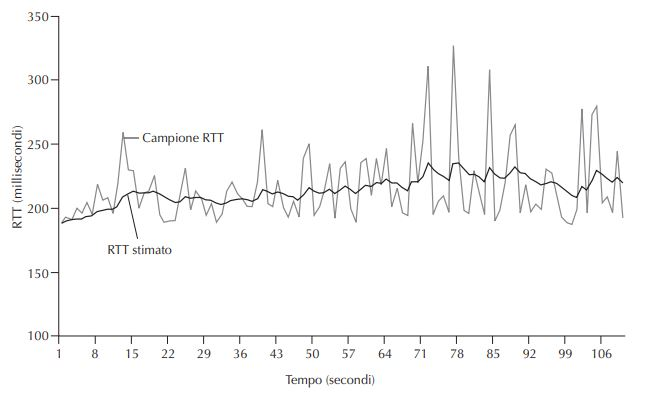
\includegraphics[width=10cm]{images/stima-rtt.JPG}
    \caption{Campioni e stima RTT}
    \label{fig:stima-rtt}
\end{figure}

La Figura \ref{fig:stima-rtt} mostra i valori SampleRTT ed EstimatedRTT con $\alpha$ = 1/8 per una connessione TCP tra \texttt{gaia.cs.umass.edu} (ad Amherst, Massachusetts) e \texttt{fantasia.eurecom.fr} (nel sud della Francia). Come si può vedere, le variazioni di SampleRTT vengono “smussate” dal calcolo di EstimatedRTT. Oltre ad avere una stima di RTT, è anche importante possedere la misura della sua variabilità, definisce la variazione RTT, DevRTT, come una stima di quanto SampleRTT generalmente si discosta da EstimatedRTT:

\begin{equation*}
    DevRTT = (1 – \beta) * DevRTT + \beta * | SampleRTT – EstimatedRTT |    
\end{equation*}

Si noti che DevRTT è un EWMA della differenza tra SampleRTT e EstimatedRTT. Se i valori di SampleRTT presentano fluttuazioni limitate, allora DevRTT sarà piccolo; in caso di notevoli fluttuazioni, DevRTT sarà grande. Il valore suggerito per $\beta$ è 0,25.

\subsubsection{Impostazione e gestione del timeout di ritrasmissione}
Dati i valori di EstimatedRTT e DevRTT, quali valori andrebbero usati per l’intervallo di timeout di TCP? Chiaramente, l’intervallo non può essere inferiore a quello di EstimatedRTT, altrimenti verrebbero inviate ritrasmissioni non necessarie. Ma l’intervallo stesso non dovrebbe essere molto maggiore di EstimatedRTT, altrimenti TCP non ritrasmetterebbe rapidamente il segmento perduto, il che comporterebbe gravi ritardi sul trasferimento dei dati. E' pertanto auspicabile impostare il timeout a EstimatedRTT più un certo margine che dovrebbe essere grande quando c’è molta fluttuazione nei valori di SampleRTT e piccolo in caso contrario. Qui entra in gioco il valore di DevRTT. Tutti questi aspetti vengono presi in considerazione dal modo in cui TCP determina l’intervallo di timeout di ritrasmissione:

\begin{equation*}
    TimeoutInterval = EstimatedRTT + 4 * DevRTT    
\end{equation*}

Viene raccomandato un valore iniziale di TimeoutInterval pari a 1 secondo. Inoltre, quando si verifica un timeout, TimeoutInterval viene raddoppiato per evitare un timeout prematuro riferito a un segmento successivo per cui si riceverà presto un acknowledgment. Tuttavia, appena viene ricevuto un segmento ed EstimatedRTT viene aggiornato, TimeoutInterval viene ricalcolato secondo la formula precedente.